% Chapter converted from: N. G. Polson, "Polya Inverse Gamma Posteriors, Fisher's Species Model,
% and Good's Predictive Rule for the Ewens Sampling Problem" (SSRN 7127198), with the companion
% note "Polya Inverse Gamma Augmentation for the Ewens Sampling Formula" folded in as a section.
% Second revision: numbers checked by code/pig_rev/*.py; figures made by code/pig_rev/make_figures.py.
% Macros: none chapter specific.
\chapter{P\'olya Inverse Gamma Posteriors, Fisher's Species Model, and Good's Predictive Rule for the Ewens Sampling Problem}\label{ch:pig}
\chaptermark{PIG and the Ewens Sampling Problem}

\begin{chaptersummary}
\citet{pig:mccullagh2016} observes that \citet{pig:fisher1943} almost discovered the Ewens sampling formula and that \citet{pig:good1953} and \citet{pig:goodtoulmin1956} asked the right predictive questions but closed neither. This chapter gives an inferential account that connects the two through P\'olya inverse gamma (PIG) augmentation \citep{pig:he2022}. Three points organise it. First, the Ewens richness likelihood is a regular one parameter natural exponential family in $\log\theta$ with cumulant $\log\{\Gamma(\theta+n)/\Gamma(\theta)\}$ and sufficient statistic $K$, the number of species; the maximum likelihood equation is pure moment matching, $K=\E[K\mid\theta]$, and a Bernstein and von Mises argument shows that the Bayes point estimator agrees with the maximum likelihood estimate to relative order $O(1/K)$ and the credible interval with the Wald interval to leading order. In this precise sense the Bayes estimator of $\theta$ sheds little light. Second, Fisher's two parameters map exactly onto the two PIG representations: the richness $\theta$ needs only the gamma ratio (Beta) block $\Gamma(\theta)/\Gamma(\theta+n)$, while the shape $\nu$ that governs departure from the log series or Ewens limit is a reciprocal gamma $1/\Gamma(\nu)$ problem requiring the full PIG(0) engine. The gamma subordinator, the prototypical generalized gamma convolution, is the structure common to Fisher's model, the Ewens partition, and PIG. Third, Good's nonparametric estimator, once given a parametric skeleton, collapses exactly to the Chinese restaurant rule $\E[q_r\mid\text{data}]=r/(n+\theta)$, so the PIG posterior yields a fully Bayesian Good Turing smoothing with honest bands. Worked examples on small cases, on Corbet's Malayan butterflies and on Williams' Rothamsted Macrolepidoptera reproduce Williams' fit ($\hat\theta=40.146$) and the temporal homogeneity check (58 expected new species against 62 observed), check the PIG(0) simulator against $e^{-\gamma s}/\Gamma(1+s)$ to within $0.07\%$, and show the Beta augmentation sampler delivering about seven times the effective samples per second of random walk Metropolis, and about half that when the random walk proposal is optimally scaled.
\end{chaptersummary}

\section{Introduction}\label{pig:sec:intro}

A sample of $n$ specimens from a large population falls into $K$ distinct species. Writing $a_j$ for the number of species represented exactly $j$ times, the abundance vector $a=(a_1,\dots,a_n)$ satisfies $\sum_j a_j=K$ and $\sum_j j a_j=n$. \citet{pig:fisher1943} modelled the frequency of frequencies and, with Corbet's Malayan butterflies and Williams' Rothamsted Macrolepidoptera, introduced a richness index that we now recognise as the parameter $\theta$ of the Ewens sampling formula \citep{pig:ewens1972}. In population genetics the same $\theta=4M\mu$ is the scaled mutation rate, the species are allele types, and $a_j$ counts the alleles carried by exactly $j$ of the $n$ sampled genes. \citet{pig:mccullagh2016} shows that Fisher's two parameter Poisson process model contains the Ewens distribution as the conditional law of $a$ given $n$, so that Fisher ``had it in his grasp'', and that \citet{pig:good1953} and \citet{pig:goodtoulmin1956}, who pioneered sequential prediction of new species, missed the Chinese restaurant description for want of a parametric skeleton.

The history repays a moment's attention because it explains what is and is not at stake. Fisher was handed a table of frequencies of frequencies, the counts $a_1,a_2,\dots$ of species seen once, twice, and so on, and asked how many species the population holds. His answer, the index of diversity, is the modern $\theta$, and his log series curve fits the Malayan and Rothamsted data strikingly well. What Fisher did not write down is the exchangeable partition process whose one step ahead rule, the probability $\theta/(n+\theta)$ that the next specimen is new, generates the whole distribution. Good and Toulmin, working a decade later on the same prediction problem, built nonparametric estimators of exactly that quantity but declined to name a model, so their formulas never simplified. Ewens, arriving from population genetics, wrote the distribution in one line. The three approaches are a single object seen from estimation, prediction, and combinatorics, and the modern task is less to choose among them than to say precisely how they fit together and where a Bayesian treatment adds something the others lack.

We revisit the problem from the standpoint of P\'olya inverse gamma augmentation \citep{pig:he2022}, a data augmentation calculus for densities in which a parameter is nested inside gamma functions. The Ewens richness likelihood is $L(\theta)\propto\theta^K\,\Gamma(\theta)/\Gamma(\theta+n)$, a gamma ratio in $\theta$; Fisher's second parameter enters through a reciprocal gamma $1/\Gamma(\nu)$; and Good's smoothing is a ratio of expected multiplicities. All three are PIG objects, and organising them this way makes precise both what Bayesian inference contributes and what it does not. The organising claim is a division of labour. The richness $\theta$ is estimated almost as well by maximum likelihood as by any Bayesian rule, because the model reduces to a one parameter exponential family whose only statistic is the species count $K$, and $K$ accumulates information slowly. Fisher's shape $\nu$ and every predictive quantity, by contrast, live where the posterior genuinely matters, and it is there that the PIG machinery earns its place.

\paragraph{What the chapter does.} Section~\ref{pig:sec:nef} shows that the Ewens richness likelihood is a regular natural exponential family (NEF) in $\varphi=\log\theta$ with sufficient statistic $K$, so that maximum likelihood is moment matching, and works the case $n=4$ by hand. Section~\ref{pig:sec:pig} sets out the two PIG representations, the Beta block for the gamma ratio and the PIG(0) block for a reciprocal gamma, and runs the resulting Gibbs sampler on a small sample line by line. Section~\ref{pig:sec:fisher} places Fisher's model, Kingman's Ewens partition, and the PIG calculus inside one gamma subordinator. Section~\ref{pig:sec:good} proves that Good's estimator collapses to $r/(n+\theta)$ and applies a Bayesian Good Turing rule to Corbet's butterflies. Section~\ref{pig:sec:bvm} states the Bernstein and von Mises theorem that makes the Bayes estimator of $\theta$ redundant, with a table across $K$. Section~\ref{pig:sec:tails} studies the two regimes, small $K$ and $K$ near $n$, where the posterior is strongly skewed, and heavy tailed when $K$ is near $n$, and recommends a weakly informative prior in the PIG family. Section~\ref{pig:sec:twovariances} untangles the two variances of the species count that appear in Fisher's and Ewens' treatments and gives an exact Gibbs sampler under a heavy tailed prior. Section~\ref{pig:sec:numerical} collects the simulation checks and the Williams analysis, Section~\ref{pig:sec:discussion} discusses, and the proofs, sampler details and exercises close the chapter.

\section{The Ewens richness model as a natural exponential family}\label{pig:sec:nef}\sectionmark{The Ewens model as an exponential family}

This section shows that all the information about richness in a sample is carried by one number, the species count $K$, and that the model is the simplest kind of exponential family. Everything later in the chapter, the samplers, the Bernstein and von Mises statement, and the heavy tails, rests on this structure.

The Ewens sampling formula assigns the abundance vector the probability
\begin{equation}\label{pig:eq:esf}
\begin{gathered}
p(a\mid\theta)=\frac{n!}{(\theta)_{(n)}}\prod_{j=1}^{n}\frac{1}{a_j!}\Bigl(\frac{\theta}{j}\Bigr)^{a_j},\\
(\theta)_{(n)}=\theta(\theta+1)\cdots(\theta+n-1)=\frac{\Gamma(\theta+n)}{\Gamma(\theta)}.
\end{gathered}
\end{equation}
Isolating $\theta$ gives $L(\theta)\propto\theta^K\,\Gamma(\theta)/\Gamma(\theta+n)$, so $K=\sum_j a_j$ is minimal sufficient: given $K$ the abundance profile has a distribution free of $\theta$, and all information about richness is the single count $K$. This is the Fisher Neyman factorisation at work and, as we now record, the whole model is a one parameter exponential family.

\begin{example}[The Ewens formula for four genes]\label{pig:ex:n4}
Take $n=4$. There are five abundance vectors, one for each way of writing $4$ as a sum of positive integers, and \eqref{pig:eq:esf} gives the probabilities in Table~\ref{pig:tab:n4}. At $\theta=1$ the rising factorial is $(1)_{(4)}=24$ and the formula reduces to the cycle type law of a uniformly random permutation of four objects: there are $1$, $6$, $3$, $8$ and $6$ permutations with the five cycle types, and the probabilities are these counts divided by $24$. At $\theta=2$ the rising factorial is $2\cdot3\cdot4\cdot5=120$ and the mass shifts toward many species. In both columns the probabilities add to one, and the mean number of species, $\sum_a K(a)\,p(a\mid\theta)$, equals $\sum_{i=0}^{3}\theta/(\theta+i)$: $1+\tfrac12+\tfrac13+\tfrac14=25/12\approx2.083$ at $\theta=1$ and $1+\tfrac23+\tfrac24+\tfrac25=2.567$ at $\theta=2$. Reading the table down the $K$ column shows sufficiency at work: the two vectors with $K=2$, namely $(0,2,0,0)$ and $(1,0,1,0)$, have probabilities in the fixed ratio $3:8$ at every $\theta$, because $\theta$ enters both only through $\theta^2/(\theta)_{(4)}$.
\end{example}

\begin{table}[t]
\centering
\caption{The Ewens sampling formula for $n=4$. The numerator column is $n!\prod_j(\theta/j)^{a_j}/a_j!$ evaluated at the stated $\theta$; dividing by $(\theta)_{(4)}$ gives the probability.}
\label{pig:tab:n4}
\small
\begin{tabular}{@{}lcccccc@{}}
\toprule
$a=(a_1,a_2,a_3,a_4)$ & $K$ & general numerator & \multicolumn{2}{c}{$\theta=1$} & \multicolumn{2}{c}{$\theta=2$}\\
\cmidrule(lr){4-5}\cmidrule(l){6-7}
 & & & numer. & prob. & numer. & prob.\\
\midrule
$(4,0,0,0)$ & 4 & $\theta^4$ & 1 & 0.0417 & 16 & 0.1333\\
$(2,1,0,0)$ & 3 & $6\theta^3$ & 6 & 0.2500 & 48 & 0.4000\\
$(0,2,0,0)$ & 2 & $3\theta^2$ & 3 & 0.1250 & 12 & 0.1000\\
$(1,0,1,0)$ & 2 & $8\theta^2$ & 8 & 0.3333 & 32 & 0.2667\\
$(0,0,0,1)$ & 1 & $6\theta$ & 6 & 0.2500 & 12 & 0.1000\\
\midrule
total & & $(\theta)_{(4)}$ & 24 & 1 & 120 & 1\\
\bottomrule
\end{tabular}
\end{table}

The intuition for the next result is that a likelihood of the form $\theta^K\times(\text{function of }\theta)$ is an exponential family in $\log\theta$, so its cumulant function delivers the mean and variance of $K$ by differentiation.

\begin{proposition}[NEF structure]\label{pig:prop:nef}
With natural parameter $\varphi=\log\theta$ and statistic $K$, \eqref{pig:eq:esf} is a regular NEF, $p(a\mid\varphi)=h(a)\exp\{\varphi K-A(\varphi)\}$, with cumulant
\[
A(\varphi)=\log\frac{\Gamma(e^{\varphi}+n)}{\Gamma(e^{\varphi})}=\log(\theta)_{(n)}.
\]
Its derivatives are $A'(\varphi)=\theta[\psi(\theta+n)-\psi(\theta)]=\E[K\mid\theta]$ and $A''(\varphi)=\Var(K\mid\theta)=\sum_{i=0}^{n-1}\frac{\theta i}{(\theta+i)^2}>0$ for $n\ge2$, where $\psi=\Gamma'/\Gamma$. Hence $\log L$ is strictly concave in $\varphi$, the maximum likelihood estimate (MLE) is unique when $1<K<n$, and it solves the moment equation
\begin{equation}\label{pig:eq:moment}
K=\theta[\psi(\theta+n)-\psi(\theta)]=\E[K\mid\theta],
\end{equation}
and the Fisher information in $\theta$ is $I(\theta)=\Var(K\mid\theta)/\theta^2=\theta^{-1}\sum_{i=0}^{n-1}i/(\theta+i)^2$.
\end{proposition}

The Feller coupling writes $K=\sum_{i=0}^{n-1}B_i$ with independent $B_i\sim\mathrm{Bernoulli}(\theta/(\theta+i))$, from which the moments in Proposition~\ref{pig:prop:nef} follow at once; the proof is in Section~\ref{pig:sec:proofs}. Equation~\eqref{pig:eq:moment} is the exponential family identity ``observed $=$ expected'': the MLE sets the number of species equal to its mean. Since $\E[K\mid\theta]$ increases continuously from $1$ (as $\theta\to0$) to $n$ (as $\theta\to\infty$), the equation has a finite positive root exactly when $1<K<n$; at the boundaries $K=1$ and $K=n$ the MLE is $0$ or $+\infty$, a fact that returns with force in Section~\ref{pig:sec:tails}.

The coupling is worth reading directly, because it is the mechanism behind every result in the chapter. Imagine the specimens arriving one at a time. The arrival that finds $i$ specimens already seated either founds a new species with probability $\theta/(\theta+i)$ or joins an old one; the indicator $B_i$ of founding is independent across $i$ because the Chinese restaurant rule depends only on the count $i$, not on the configuration. The number of species is then a sum of independent coin flips whose success probabilities decay like $\theta/i$, so $K$ behaves like $\theta\sum_{i<n}1/i\approx\theta\log n$: information about $\theta$ enters one nearly fair coin at the start and progressively rarer coins thereafter. Sufficiency of $K$ now has a plain reading. Two samples with the same species count carry identical evidence about richness however differently their specimens are distributed among species, because given the sequence of founding events the way later specimens join old species does not involve $\theta$. The moment equation~\eqref{pig:eq:moment} inherits the same simplicity: since the log likelihood is concave in $\varphi=\log\theta$ with curvature equal to $\Var(K)$, there is a single hump, no multimodality to worry a sampler, and the MLE is found by matching one number.

\begin{example}[Moments by coin flips]\label{pig:ex:feller}
For $n=4$ and $\theta=1$ the coins have success probabilities $1,\tfrac12,\tfrac13,\tfrac14$, so $\E[K]=25/12$ and $\Var(K)=0+\tfrac14+\tfrac29+\tfrac{3}{16}=0.6597$, which agrees with the variance computed from the $\theta=1$ column of Table~\ref{pig:tab:n4}. For a sample of $n=50$ with $K=10$ species, solving~\eqref{pig:eq:moment} numerically gives $\hat\theta=3.480$; at that value $\Var(K\mid\hat\theta)=6.20$, so $I(\hat\theta)=6.20/3.480^2=0.512$ and the standard error is $I(\hat\theta)^{-1/2}=1.40$. Ten species in fifty specimens therefore pin $\theta$ down only to within a factor of about two either way. Note how much smaller $\Var(K)=6.20$ is than $\E[K]=10$: the coins with large $i$ are rarely heads, and a sum of rare Bernoulli variables has variance below its mean.
\end{example}

\paragraph{Conjugate prior.} The NEF carries a Diaconis and Ylvisaker conjugate family \citep{pig:diaconis1979}. For $n_0>1$, $\tau>0$ and $\tau-1<\kappa<\tau n_0-1$,
\begin{equation}\label{pig:eq:conj}
\pi(\theta\mid\kappa,\tau,n_0)\;\propto\;\theta^{\kappa}\Bigl[\frac{\Gamma(\theta)}{\Gamma(\theta+n_0)}\Bigr]^{\tau},
\end{equation}
which is proper (Section~\ref{pig:sec:proofs}) and reads as $\tau$ prior Ewens samples of size $n_0$ displaying $\kappa$ species in total, measured against the base measure $\dd\theta$. Given independent samples $(n_j,K_j)_{j=1}^{J}$ the posterior is $\pi(\theta\mid\text{data})\propto\theta^{\kappa+K_\bullet}[\Gamma(\theta)/\Gamma(\theta+n_0)]^{\tau}\prod_j\Gamma(\theta)/\Gamma(\theta+n_j)$ with $K_\bullet=\sum_j K_j$, closed in the family when the $n_j$ are all equal to $n_0$. In practice we default to a diffuse gamma prior, which is not conjugate but is handled \emph{exactly} by the augmentation of the next section. Throughout the chapter the ``diffuse prior'' is $\mathrm{Ga}(10^{-2},10^{-2})$ unless stated otherwise.

\paragraph{The information grows logarithmically.} The Feller representation gives the \citet{pig:korwar1973} law of large numbers, $K/\log n\to\theta$ almost surely, and a central limit theorem $K\approx\mathcal{N}(\theta\log n,\theta\log n)$. Since $\E[K]=\theta[\psi(\theta+n)-\psi(\theta)]=\theta\log n-\theta\psi(\theta)+o(1)$, the effective number of observations for $\theta$ is $K$ itself, which grows only like $\log n$: even Williams' $n=15{,}609$ specimens supply just $K=240$ effective data points, and $K/\log n=24.9$ still sits well below $\theta=40$ because convergence is logarithmically slow. This is the quantitative reason the richness parameter is hard to pin down no matter how many specimens are collected, and the backdrop for the Bernstein and von Mises statement of Section~\ref{pig:sec:bvm}. In genetic terms, sequencing ten times as many genes from a neutral population adds only about $\theta\log10\approx2.3\,\theta$ new allele types, and so only that many new effective observations on the mutation rate.

\section{P\'olya inverse gamma augmentation: two representations}\label{pig:sec:pig}\sectionmark{Two PIG representations}

This section supplies the computational tool. The obstruction to conjugacy is that $\theta$ sits inside a gamma ratio, and \citet{pig:he2022} give two integral representations that remove such obstructions; the Ewens problem uses the first, Fisher's second parameter the second.

The idea of data augmentation is to trade a hard density for a tractable joint density with an extra latent variable, so that each conditional is a standard draw. A density is awkward when its normaliser or a factor cannot be written in closed exponential family form; the trick is to represent that factor as an expectation over a latent variable chosen so that, given the latent, the target becomes conjugate. The gamma ratio $\Gamma(\theta)/\Gamma(\theta+n)$ and the reciprocal $1/\Gamma(\nu)$ are the two shapes in which a gamma function can trap a parameter, and PIG supplies a latent for each. What makes the calculus attractive here is that the latents are elementary, a Beta variable in the first case and an infinitely divisible positive variable in the second, so the resulting samplers avoid any evaluation of $\Gamma$ or its logarithm inside the inner loop and mix close to independently.

\paragraph{R1: the gamma ratio (Beta block).} The ratio in \eqref{pig:eq:esf} has the Beta representation, row three of Table 2 in \citet{pig:he2022},
\begin{equation}\label{pig:eq:beta}
\frac{\Gamma(\theta)}{\Gamma(\theta+n)}=\frac{1}{\Gamma(n)}\int_0^1\eta^{\theta-1}(1-\eta)^{n-1}\dd\eta,
\end{equation}
which is nothing more than the Beta integral $B(\theta,n)=\Gamma(\theta)\Gamma(n)/\Gamma(\theta+n)$ divided by $\Gamma(n)$. The factor $\eta^{\theta-1}=e^{(\theta-1)\log\eta}$ is exponential in $\theta$, which is the whole point. Under a $\mathrm{Ga}(a_0,b_0)$ prior the augmented posterior $p(\theta,\eta\mid K)\propto\theta^{K+a_0-1}e^{-b_0\theta}\eta^{\theta-1}(1-\eta)^{n-1}$ has the original posterior as its $\theta$ marginal and gives the two block Gibbs sampler
\begin{equation}\label{pig:eq:gibbs}
\theta\mid\eta\sim\mathrm{Ga}\bigl(K+a_0,\;b_0-\log\eta\bigr),\qquad\eta\mid\theta\sim\mathrm{Be}(\theta,n),
\end{equation}
both draws standard, no gamma function evaluation required. This is a variant of the \citet{pig:escobar1995} augmentation for the Dirichlet process concentration; each factor $\Gamma(\theta)/\Gamma(\theta+n_j)$ contributes one latent $\eta_j$, so the multisample posterior of \eqref{pig:eq:conj} needs one Beta draw per sample.

\begin{example}[Checking the Beta identity]\label{pig:ex:betaid}
At $\theta=2.5$, $n=10$ the left side of~\eqref{pig:eq:beta} is $\Gamma(2.5)/\Gamma(12.5)=9.7143\times10^{-9}$, and numerical integration of the right side returns the same value to a relative error below $10^{-9}$. At the Williams scale, $\theta=40.146$ and $n=50$, both sides equal $1.0967\times10^{-90}$; at $\theta=0.5$, $n=5$ both equal $(0.5\cdot1.5\cdot2.5\cdot3.5\cdot4.5)^{-1}=0.033862$. The latent $\eta$ has a direct meaning: since $\E[-\log\eta\mid\theta]=\psi(\theta+n)-\psi(\theta)$, the gamma rate $b_0-\log\eta$ in~\eqref{pig:eq:gibbs} is a one draw estimate of $\E[K\mid\theta]/\theta$, and the Gibbs step for $\theta$ is a randomised version of the moment equation~\eqref{pig:eq:moment}.
\end{example}

\begin{example}[The Beta augmentation sampler, line by line]\label{pig:ex:gibbs}
Take $n=50$, $K=10$ and the diffuse prior $a_0=b_0=0.01$, and start the chain at $\theta^{(0)}=1$. Each iteration draws $\eta\sim\mathrm{Be}(\theta,50)$, forms the rate $0.01-\log\eta$, and draws $\theta\sim\mathrm{Ga}(10.01,\text{rate})$. Table~\ref{pig:tab:gibbs} lists the first six iterations from one run. The conditional mean $10.01/\text{rate}$ moves from $1.7$ to about $3.9$ within three steps, the chain forgets its poor starting value at once, and the draws scatter around the posterior centre. Over $99{,}000$ further iterations the chain gives posterior mean $3.596$, standard deviation $1.468$ and central $95\%$ interval $[1.43, 7.11]$, against $3.602$, $1.469$ and $[1.43, 7.10]$ from exact quadrature of $\theta^{K+a_0-1}e^{-b_0\theta}\Gamma(\theta)/\Gamma(\theta+n)$. The integrated autocorrelation time is $2.1$, so each draw is worth about half an independent one. The posterior mean sits above the MLE $3.480$ and the interval is lopsided about it, $[\hat\theta-2.05,\hat\theta+3.62]$, a first sign of the right skew studied in Section~\ref{pig:sec:tails}.
\end{example}

\begin{table}[t]
\centering
\caption{First six iterations of the Beta augmentation sampler~\eqref{pig:eq:gibbs} for $n=50$, $K=10$, prior $\mathrm{Ga}(0.01,0.01)$, started at $\theta^{(0)}=1$.}
\label{pig:tab:gibbs}
\small
\begin{tabular}{@{}ccccc@{}}
\toprule
$t$ & $\eta^{(t)}\sim\mathrm{Be}(\theta^{(t-1)},50)$ & rate $0.01-\log\eta^{(t)}$ & $\E[\theta\mid\eta^{(t)}]=10.01/\text{rate}$ & $\theta^{(t)}$\\
\midrule
1 & 0.0029 & 5.857 & 1.709 & 2.510\\
2 & 0.0331 & 3.419 & 2.928 & 2.630\\
3 & 0.0607 & 2.813 & 3.559 & 2.805\\
4 & 0.0781 & 2.560 & 3.910 & 4.635\\
5 & 0.0591 & 2.838 & 3.527 & 5.111\\
6 & 0.0796 & 2.541 & 3.939 & 5.377\\
\bottomrule
\end{tabular}
\end{table}

\begin{remark}[Drawing $\eta$ when $\theta$ is small]\label{pig:rem:smallbeta}
When $K$ is small the chain visits values of $\theta$ near zero, where a $\mathrm{Be}(\theta,n)$ draw can underflow to $\eta=0$ in floating point and the rate $-\log\eta$ becomes infinite. The sampler needs only $\log\eta$, which is computed stably as $\log\eta=\log G_1-\log(G_1+G_2)$ with $G_2\sim\mathrm{Ga}(n,1)$ and $\log G_1=\log G'+(\log U)/\theta$, $G'\sim\mathrm{Ga}(\theta+1,1)$, $U\sim\mathrm{U}(0,1)$, using the identity $G'U^{1/\theta}\sim\mathrm{Ga}(\theta,1)$. All chains in this chapter are run this way.
\end{remark}

\paragraph{R2: the reciprocal gamma (PIG(0) block).} When a parameter appears as $1/\Gamma(\alpha)$ rather than in a fixed $n$ ratio, the relevant object is the P\'olya inverse gamma law of \citet[Definition 2.1]{pig:he2022}: $X_0\sim\mathrm{PIG}(0)$ if and only if
\begin{equation}\label{pig:eq:pig0}
\E\bigl[e^{-s^2X_0}\bigr]=\frac{e^{-\gamma s}}{\Gamma(1+s)},\qquad s>0,
\end{equation}
with $\gamma$ the Euler Mascheroni constant. Rearranged, $1/\Gamma(\nu)=\nu\,e^{\gamma\nu}\,\E[e^{-\nu^2X_0}]$, so a reciprocal gamma factor becomes an average of Gaussian kernels in $\nu$, and given $X_0$ the parameter $\nu$ enters the augmented density through $e^{\gamma\nu-\nu^2X_0}$. The next proposition, which is Theorem 1 of \citet{pig:he2022} with a short self contained proof in Section~\ref{pig:sec:proofs}, makes $X_0$ simulable.

\begin{proposition}[Inverse gamma series for PIG(0)]\label{pig:prop:pig0}
Let $Y_1,Y_2,\dots$ be independent $\mathrm{InvGa}(3/2,1)$ variables, that is $1/Y_k\sim\mathrm{Ga}(3/2,1)$. Then $X_0=\sum_{k\ge1}Y_k/(4k^2)$ converges almost surely and satisfies~\eqref{pig:eq:pig0}. In particular $\E[X_0]=\sum_k 1/(2k^2)=\zeta(2)/2=\pi^2/12$, while $\Var(X_0)=\infty$.
\end{proposition}

The intuition is that each inverse gamma term contributes one Weierstrass factor $(1+s/k)e^{-s/k}$ of $1/\Gamma(1+s)$, and the infinite product of these factors is exactly $e^{-\gamma s}/\Gamma(1+s)$. Representation R2 is what one needs for Fisher's shape $\nu$ and for the vector concentration $\alpha=(\alpha_1,\dots,\alpha_K)$ of the finite Dirichlet multinomial \citep[Section 4.3]{pig:he2022}, where individual factors $1/\Gamma(\alpha_k)$ appear. The infinite variance is worth noticing: $X_0$ is itself heavy tailed, so its sample mean settles slowly, as Section~\ref{pig:sec:numerical} shows.

\begin{remark}\label{pig:rem:r1}
The scalar Ewens richness problem needs only R1. That the harder representation R2 is unnecessary here is the computational shadow of the inferential fact, made precise in Section~\ref{pig:sec:bvm}, that the Bayes estimator of $\theta$ adds little.
\end{remark}

\section{Fisher's two parameters and the gamma subordinator picture}\label{pig:sec:fisher}\sectionmark{Fisher's two parameters}

This section explains why the Ewens partition, Fisher's log series, and the PIG calculus are one object, and it identifies which of Fisher's two parameters calls for which PIG representation.

Fisher's model posits species intensities $\lambda$ distributed as a Poisson process with a gamma mean measure $G$ on $(0,\infty)$, and $\mathrm{Poisson}(\lambda)$ specimen counts. Concretely $G(\dd\lambda)=c\,\lambda^{\nu-1}e^{-\lambda/\beta}\dd\lambda$ with shape $\nu$, scale $\beta$ and a constant $c$ that we absorb into $\theta$. The joint intensity and count process is $Z\sim\mathrm{PP}(\mu)$ with $\mu(\mathrm{d}\lambda,r)=e^{-\lambda}\lambda^r/r!\;G(\mathrm{d}\lambda)$, and the frequency of frequencies $m_r=\#\{\lambda:(\lambda,r)\in Z\}$ is Poisson with
\begin{equation}\label{pig:eq:nbseries}
\mu_r=\E[m_r]=\theta\,\frac{\Gamma(r+\nu)}{r!\,\Gamma(\nu)}\,x^r(1-x)^{\nu},\qquad r\ge1,\qquad x=\frac{\beta}{1+\beta},
\end{equation}
a negative binomial series \citep{pig:mccullagh2016}. As $\nu\to0$, with $\theta$ held fixed in this parametrisation, $\Gamma(r+\nu)/\Gamma(\nu)\sim\nu\,(r-1)!$; absorbing the factor $\nu$ into $\theta$ gives $\mu_r\to\theta x^r/r$, Fisher's log series, with total specimen count $N=\sum_{r\ge1}r\,m_r$ and species count $K=\sum_{r\ge1}m_r$ having means $\E[N]=\theta x/(1-x)$ and $\E[K]=-\theta\log(1-x)$. Eliminating $x$ between the last two gives Fisher's famous relation $\E[K]=\theta\log(1+\E[N]/\theta)$ \citep{pig:fisher1943}. Fisher concluded from the butterfly data that $\nu\approx0$.

\paragraph{The common structure.} The gamma subordinator $\{G_t\}_{t\ge0}$ has L\'evy measure $\rho(\mathrm{d}\lambda)=\lambda^{-1}e^{-\lambda}\dd\lambda$, the prototypical generalized gamma convolution (GGC) with a degenerate Thorin measure \citep{pig:bondesson1992}. Normalising by the total mass $G_\theta\sim\mathrm{Ga}(\theta,1)$ yields the Dirichlet process \citep{pig:ferguson1973}, whose sample partition is $\mathrm{Ewens}(\theta)$ \citep{pig:kingman1978}. The log series multiplicities $\mu_r\propto x^r/r$ are the discretised L\'evy density of that subordinator, and $m_r\sim\mathrm{Po}(\mu_r)$ is exactly the \citet{pig:arratia1992} Poisson process approximation. The GGC calculus that PIG uses to build augmentations \citep[Remark 4]{pig:he2022} is therefore the same calculus that generates the Fisher and Ewens model, so the two are not analogies but one object.

It is worth tracing the chain slowly, since it is what licenses treating estimation, prediction, and combinatorics as one problem. A subordinator is a nondecreasing process built by summing a Poisson rain of positive jumps, and the gamma subordinator is the case where a jump of size near $\lambda$ arrives at rate $\lambda^{-1}e^{-\lambda}$. Small jumps are abundant and large jumps rare, and the weight $\lambda^{-1}$ near the origin is precisely what makes infinitely many tiny species possible in a finite population. Read the jumps of $G_\theta$ as the unnormalised abundances of the species and divide by the total mass: the resulting random probability vector is a draw from the Dirichlet process, and a sample of $n$ specimens from it partitions into species according to the Ewens formula~\eqref{pig:eq:esf}. The mass parameter $\theta$ of the subordinator is the richness parameter of the partition, one quantity wearing two hats. Now count, rather than normalise. If each species of intensity $\lambda$ contributes $\mathrm{Poisson}(\lambda)$ specimens, the number of species represented exactly $r$ times is itself Poisson, with mean obtained by integrating the jump rate against the Poisson weight. Carrying out the integral for the scaled jump rate $\theta\lambda^{-1}e^{-\lambda/\beta}$,
\[
\int_0^\infty\frac{e^{-\lambda}\lambda^r}{r!}\,\theta\lambda^{-1}e^{-\lambda/\beta}\dd\lambda=\frac{\theta\,(r-1)!}{r!}\Bigl(\frac{\beta}{1+\beta}\Bigr)^{r}=\frac{\theta x^r}{r},
\]
returns Fisher's log series. So Fisher's frequency of frequencies curve, Kingman's partition, and Ferguson's process are three exposures of the same gamma photograph, and the Thorin measure that indexes the PIG family is the dial that was set to a point mass all along. The practical consequence is the parameter map below: moving the Thorin dial off its point mass, which is what a nonzero $\nu$ does, is exactly the reciprocal gamma problem R2 solves.

\paragraph{The parameter map.} Fisher's two parameters split cleanly across the two PIG representations, and across the three worked examples of \citet{pig:he2022}:
\begin{center}
\footnotesize
\begin{tabular}{@{}>{\raggedright\arraybackslash}p{0.27\textwidth}>{\raggedright\arraybackslash}p{0.33\textwidth}>{\raggedright\arraybackslash}p{0.3\textwidth}@{}}
\toprule
Fisher parameter & PIG representation & He, Polson and Xu example\\
\midrule
richness or mass $\theta$ & R1 gamma ratio $\Gamma(\theta)/\Gamma(\theta+n)$ & Dirichlet concentration (Section 4.3)\\
shape $\nu$, departure from log series & R2 reciprocal gamma $1/\Gamma(\nu)$ & gamma shape, negative binomial dispersion (Sections 4.1 and 4.2)\\
\bottomrule
\end{tabular}
\end{center}
Inference for $\theta$ is the near trivial NEF problem of Section~\ref{pig:sec:nef}; inference for $\nu$ is a genuine gamma shape problem that only R2 renders a clean Gibbs step.

\paragraph{Two parameter Pitman and Yor.} The natural discrete parameter analogue of Fisher's richness and shape pair is the two parameter Poisson Dirichlet process $(\theta,\sigma)$, $0\le\sigma<1$, $\theta>-\sigma$ \citep{pig:pitman2006}, with sequential predictive rule
\begin{equation}\label{pig:eq:py}
\begin{gathered}
\Pr(\text{new species})=\frac{\theta+\sigma K}{n+\theta},\\
\Pr(\text{join species seen } n_j \text{ times})=\frac{n_j-\sigma}{n+\theta}.
\end{gathered}
\end{equation}
Setting $\sigma=0$ recovers the Ewens rule $\theta/(n+\theta)$ of Section~\ref{pig:sec:good}. The sampling distribution of the block sizes carries factors $\Gamma(n_j-\sigma)/\Gamma(1-\sigma)$ and $\prod_{i=1}^{K-1}(\theta+i\sigma)$, again products of gamma ratios, but they are rising factorials in the numerator, which the Beta block R1 does not remove, so Chapter~\ref{ch:esf} computes the two parameter posterior by quadrature; $\sigma$ tunes the power law tail of the species abundance curve that the one parameter Ewens model cannot fit. We record this only to place Fisher's model in the wider family and do not fit it to the butterfly data, for which McCullagh finds $\sigma$ superfluous.

\section{Good's predictive and the Ewens reconciliation}\label{pig:sec:good}\sectionmark{Good's predictive}

This section turns from estimation to prediction. It proves that Good's nonparametric estimator is the Chinese restaurant rule in disguise, gives the predictive law of new species in closed form, and works both on small cases and on Corbet's butterflies.

\citet{pig:good1953} estimated the population frequency $q_r$ of a species seen $r$ times by the nonparametric ratio
\begin{equation}\label{pig:eq:good}
\E[q_r\mid\text{data}]=\frac{r+1}{n+1}\,\frac{\mu_{r+1,\,n+1}}{\mu_{r,\,n}},\qquad\mu_{r,n}=\E[a_r(n)],
\end{equation}
the Good Turing estimator, deliberately avoiding parametric assumptions. In practice $\mu_{r,n}$ is replaced by the observed $a_r$, and the ratio $r^*=(r+1)a_{r+1}/a_r$ is called the adjusted count. Under the Ewens model the expected multiplicities are available in closed form, and \eqref{pig:eq:good} telescopes.

Good's reasoning is a small marvel of empirical Bayes and deserves stating in words. He wanted the population frequency of a species observed $r$ times but had no model for how frequencies are distributed, so he estimated it indirectly. A species seen $r$ times in a sample of $n$ would, in a sample of $n+1$, tend to be seen $r+1$ times, and the expected number of such species is $\mu_{r+1,n+1}$; dividing by the number seen $r$ times and rescaling by $(r+1)/(n+1)$ converts a ratio of observable counts into an estimate of an unobservable frequency. The construction is entirely nonparametric, which was the point, and it is why the answer arrived as a ratio of two expectations he had no way to evaluate. The moment he grants himself a model for the $\mu_{r,n}$, the ratio can be computed, and under the Ewens model it collapses.

\begin{proposition}[Good's rule is the Ewens predictive]\label{pig:prop:good}
Under \eqref{pig:eq:esf}, $\E[a_r(n)]=\dfrac{\theta}{r}\,\dfrac{n!}{(n-r)!}\,\dfrac{\Gamma(\theta+n-r)}{\Gamma(\theta+n)}$ for $1\le r\le n$, and consequently
\[
\E[q_r\mid\text{data}]=\frac{r}{n+\theta},\qquad r\ge1,
\]
with unseen mass $q_0=\theta/(n+\theta)$, the probability the next specimen is a new species.
\end{proposition}

The proof (Section~\ref{pig:sec:proofs}) is a few lines of gamma algebra; McCullagh's remark that Good ``could easily have arrived at'' $r/(n+\theta)$ is thus an identity, not an approximation. Good's insistence on nonparametric smoothing left him with \eqref{pig:eq:good} in a form that never simplified, whereas the parametric skeleton collapses it to the Chinese restaurant rule. The resulting formula is almost embarrassingly simple: the estimated frequency of a species seen $r$ times is $r/(n+\theta)$, the observed proportion $r/n$ shrunk toward zero by the factor $n/(n+\theta)$, with the mass $\theta/(n+\theta)$ freed up and assigned to species not yet seen. This is the Bayesian smoothing that Good approximated from the data alone, now with $\theta$ as the single knob controlling how much probability is held in reserve for the unseen.

\begin{example}[Good's rule by hand]\label{pig:ex:goodhand}
Take $\theta=1$ and $n=4$. Proposition~\ref{pig:prop:good} gives $\mu_{1,4}=\frac11\cdot4\cdot\Gamma(4)/\Gamma(5)=1$, which matches Table~\ref{pig:tab:n4}: the expected number of singletons is $4(1/24)+2(6/24)+1(8/24)=1$. In a sample of five, $\mu_{2,5}=\frac12\cdot20\cdot\Gamma(4)/\Gamma(6)=\frac12$. Good's ratio is $\frac{2}{5}\cdot\frac{1/2}{1}=\frac15=1/(n+\theta)$, as claimed. In the same way $\mu_{2,4}=\tfrac12$ and $\mu_{3,5}=\tfrac13$ give $\frac35\cdot\frac{1/3}{1/2}=\frac25=2/(n+\theta)$, and the unseen mass is $1/5$. The three estimates $\tfrac15$, $\tfrac25$ and the mass $\tfrac15$ for new species are exactly the Chinese restaurant probabilities for the fifth customer.
\end{example}

\paragraph{Bayesian Good Turing.} Proposition~\ref{pig:prop:good} depends on $\theta$, which the PIG posterior supplies. The Bayesian Good Turing estimate is $\E[q_r\mid K]=\E[\,r/(n+\theta)\mid K\,]$ with a posterior credible band obtained by pushing the draws \eqref{pig:eq:gibbs} through $r/(n+\theta)$. For large $n$ the relative uncertainty in $q_r=r/(n+\theta)$ is about $\mathrm{sd}(\theta)/n$, which is negligible, whereas the relative uncertainty in $q_0=\theta/(n+\theta)$ is about $\mathrm{sd}(\theta)/\theta$, which is not; the posterior matters for the unseen mass, not for the seen frequencies (Figure~\ref{pig:fig:goodturing}(b)). The \citet{pig:goodtoulmin1956} extension follows the same route and, through the Feller coupling, is available in closed form.

\begin{proposition}[Predictive law of new species]\label{pig:prop:newspecies}
Let $U_m$ be the number of new species among $m$ further specimens. Then, given $\theta$, $U_m\overset{d}{=}\sum_{i=n}^{n+m-1}B_i$ with independent $B_i\sim\mathrm{Bernoulli}(\theta/(\theta+i))$, independent of the first $n$ specimens, so
\[
\E[U_m\mid\theta]=\theta[\psi(\theta+n+m)-\psi(\theta+n)],\]
\[\Var[U_m\mid\theta]=\sum_{i=n}^{n+m-1}\frac{\theta\,i}{(\theta+i)^2}.
\]
The unconditional predictive variance adds parameter uncertainty by the law of total variance, $\Var(U_m\mid K)=\E[\Var(U_m\mid\theta)\mid K]+\Var(\E[U_m\mid\theta]\mid K)$, both terms computed from the PIG draws \eqref{pig:eq:gibbs}.
\end{proposition}

This gives the honest predictive interval of Figures~\ref{pig:fig:predictive} and~\ref{pig:fig:accumulation}, the object Good and Toulmin sought. The sampling term grows like $\theta\log(1+m/n)$ while the parameter term grows like its square, $\mathrm{sd}(\theta)^2\log^2(1+m/n)$, so the sampling term dominates for small enlargements and the parameter term for large ones, and the accumulation band widens without ever closing. For a doubling, $m=n$ with $n\gg\theta$, the mean is close to $\theta\log2$: about $27$ new species for Williams' 1933 sample.

\begin{example}[Good Turing and log series smoothing for Corbet's butterflies]\label{pig:ex:butterflies}
Corbet's Malayan butterfly collection, analysed in \citet{pig:fisher1943} and revisited by \citet[Chapter 6]{pig:efronhastie2016}, gives for $r=1,\dots,15$ the frequencies of frequencies
\[
a_r=118,\ 74,\ 44,\ 24,\ 29,\ 22,\ 20,\ 19,\ 20,\ 15,\ 12,\ 14,\ 6,\ 12,\ 6,
\]
which account for $435$ species and $2029$ specimens; we use only these fifteen cells. The raw adjusted counts $r^*=(r+1)a_{r+1}/a_r$ begin sensibly, $r^*=1.25,\ 1.78,\ 2.18$ for $r=1,2,3$, and then become erratic: $6.04$ at $r=4$, $14.0$ at $r=11$, $5.57$ at $r=12$ and $28.0$ at $r=13$, because a single small $a_r$ in the denominator can double or halve the estimate (Figure~\ref{pig:fig:butterflies}(b)). This is the well known instability of unsmoothed Good Turing.

Under Fisher's model the $a_r$ are independent Poisson counts with means $\theta x^r/r$, where $x$ is the probability parameter of~\eqref{pig:eq:nbseries} with $\nu=0$, and Good's ratio has expectation $(r+1)\mu_{r+1}/\mu_r=r x$. Smoothing therefore means estimating $x$. With a prior flat in $\log\theta$ and in $x\in(0.85,1]$, the posterior from the fifteen Poisson cells has $\theta$ mean $135.3$ with $95\%$ interval $[121.6, 150.7]$ and $x$ mean $0.993$ with interval $[0.979, 1.000]$; the fitted multiplicities $134.3,\ 66.7,\ 44.1,\ 32.9,\ 26.1,\dots$ match the data with a Pearson statistic of $13.5$ on $13$ degrees of freedom (Figure~\ref{pig:fig:butterflies}(a)). The smoothed adjusted counts are $r x$, so $r^*=0.993,\ 1.986,\ 2.979,\dots$ with $95\%$ intervals $[0.979r, 1.000r]$, about $2\%$ of $r$ wide. The truncated table identifies $\theta$ well and $x$ only weakly, as it must: $x^r$ barely varies over $r\le15$ when $x$ is close to one, which is the case $n\gg\theta$ in Ewens' notation, since $x=n/(n+\theta)$ is precisely the shrinkage factor of Proposition~\ref{pig:prop:good}.

The same posterior predicts the number of new species $U$ in a second collection of equal effort. Under the log series the expected number is $\sum_r(-1)^{r+1}\theta x^r/r=\theta\log(1+x)$ (Exercise~\ref{pig:exr:goodtoulmin}), with posterior mean $93.3$ and interval $[84.1, 103.4]$; adding the Poisson noise of the new collection gives a $95\%$ predictive interval $[73, 115]$. Good and Toulmin's nonparametric estimate is the alternating sum $\sum_r(-1)^{r+1}a_r=75$ with standard error $(\sum_r a_r)^{1/2}=20.9$. The two answers are compatible, and the difference has a clear source: the data hold $118$ singletons against the log series' $134$, a deficit of $1.4$ Poisson standard deviations, and $a_1$ is the largest cell in the alternating sum. The parametric answer is four times more precise about the mean because it borrows strength across all fifteen cells; the price is reliance on the log series shape, which the Pearson statistic does not reject.
\end{example}

\begin{figure}[t]
\centering
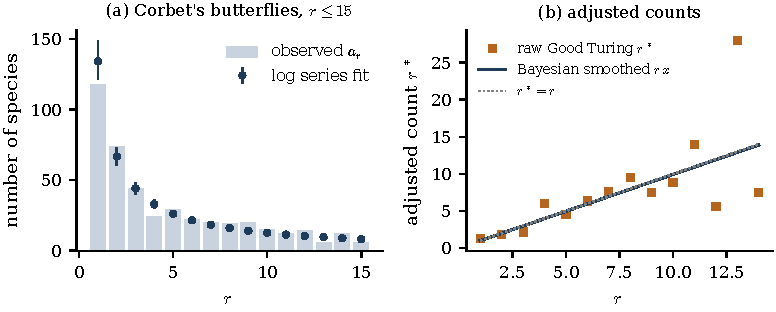
\includegraphics[width=\textwidth]{figures/pig_butterflies.pdf}
\caption{Corbet's Malayan butterflies, $r\le15$. (a) Observed frequencies of frequencies (bars) and posterior mean log series fit $\theta x^r/r$ with $95\%$ posterior intervals. (b) Raw Good Turing adjusted counts $r^*=(r+1)a_{r+1}/a_r$ (squares) against the Bayesian smoothed $r x$ (line); the dotted line is $r^*=r$.}
\label{pig:fig:butterflies}
\end{figure}

\section{The Bayes estimate of \texorpdfstring{$\theta$}{theta} sheds little; the posterior sheds light on prediction and uncertainty}\label{pig:sec:bvm}\sectionmark{The Bayes estimate sheds little}

This section makes precise the claim that, for the richness parameter itself, a Bayesian point estimate and interval add almost nothing to maximum likelihood once $K$ is moderate. The NEF structure delivers a clean Bernstein and von Mises statement. Write $\varphi=\log\theta$, $\hat\varphi$ for the MLE, and $J_n=A''(\hat\varphi)=\Var(K\mid\hat\theta)$ for the observed information in $\varphi$, which by Proposition~\ref{pig:prop:nef} is of the same order as $\E[K]=\theta[\psi(\theta+n)-\psi(\theta)]$, growing like $\theta\log n$.

Bernstein and von Mises is the theorem that, with enough information, the posterior forgets its prior and lines up with the sampling distribution of the MLE. What makes it bite cleanly here is that a one parameter exponential family has a single Fisher information $J_n$, and that $J_n$ equals the variance of the sufficient statistic $K$. The posterior for $\varphi$ is therefore a Gaussian whose width is fixed by how variable the species count is, and the prior contributes a correction of relative order $1/J_n$. The one subtlety, and the reason the phrase ``sheds little'' needs the qualifier ``estimator'', is that $J_n$ grows only logarithmically in the sample size. Doubling the number of specimens does not halve the posterior variance of $\theta$; it barely moves it. The governing quantity is $K$, and $K$ is a slow accumulator.

\begin{proposition}[Asymptotic redundancy]\label{pig:prop:bvm}
For any prior with a continuous positive density at $\hat\theta$, the posterior of $\varphi$ is asymptotically $\mathcal{N}(\hat\varphi,J_n^{-1})$ as $J_n\to\infty$. The posterior mean satisfies $\E[\theta\mid K]=\hat\theta+O(\hat\theta J_n^{-1})$, the central $95\%$ credible interval equals the Wald interval $\hat\theta\pm1.96\,I(\hat\theta)^{-1/2}$ up to $o(\hat\theta J_n^{-1/2})$, and two priors differing by a smooth reweighting give posteriors within total variation $O(J_n^{-1/2})$ and posterior means within $O(\hat\theta J_n^{-1})$.
\end{proposition}

Thus the effective sample size is $K$, not $n$: with $K=27$ the posterior already tracks the likelihood, and with Williams' $K=240$ the prior is a rounding error (Section~\ref{pig:sec:numerical}). This is the precise content of ``sheds little.'' The statement is specific to $\theta$. It does not transfer to the shape $\nu$, whose information accumulates differently, nor to prediction of unseen mass $q_0$, where the posterior over $\theta$ is exactly what supplies the uncertainty. Bayesian machinery is redundant for estimating richness and indispensable for the predictive questions that motivated Good. The distinction is not that estimation is frequentist and prediction Bayesian, but that the two questions load on different features of the model: a point estimate of $\theta$ asks for the centre of a well behaved likelihood, which any sensible method locates, whereas a predictive interval for the unseen must propagate the residual uncertainty in $\theta$, which only a posterior carries honestly.

\begin{example}[Bernstein and von Mises across $K$]\label{pig:ex:bvmtable}
Fix $n=1000$ and let the observed species count range from $K=3$ to $K=160$. Table~\ref{pig:tab:bvm} compares the MLE and Wald interval with the posterior mean and $95\%$ credible interval under the diffuse prior, all computed by exact quadrature. Three patterns are visible. First, the posterior mean is within $0.04$ standard errors of the MLE at every $K$, even $K=3$: the point estimates are interchangeable. Second, the intervals are not: at $K=3$ and $K=5$ the Wald interval runs below zero, an impossible value, while the credible interval is asymmetric about the MLE, extending $2.7$ standard errors above it but only $1.2$ below at $K=3$. Third, the disagreement fades steadily as $K$ grows, from a gross mismatch at $K=3$ to endpoint differences under $10\%$ of a standard error at $K=160$, at the rate $J_n^{-1/2}$ that Proposition~\ref{pig:prop:bvm} predicts. The Wald interval computed on the natural scale, $\hat\theta\exp(\pm1.96J_n^{-1/2})$, respects positivity and captures the direction of the asymmetry, though it overshoots on the right; at small $K$ neither Gaussian interval reproduces the credible interval, which is why Section~\ref{pig:sec:tails} recommends reporting the posterior itself, summarised on the $\log\theta$ scale.
\end{example}

\begin{table}[t]
\centering
\caption{Maximum likelihood against the diffuse prior posterior for $n=1000$ as the species count $K$ varies, by exact quadrature. $J_n=\Var(K\mid\hat\theta)$ is the information in $\log\theta$; ``log Wald'' is $\hat\theta\exp(\pm1.96J_n^{-1/2})$.}
\label{pig:tab:bvm}
\begin{adjustbox}{max width=\textwidth}
\begin{tabular}{@{}rrrrccrcr@{}}
\toprule
$K$ & $\hat\theta$ & $J_n$ & SE & Wald $95\%$ & log Wald $95\%$ & post.\ mean & credible $95\%$ & skew\\
\midrule
3 & 0.282 & 1.9 & 0.204 & $[-0.118, 0.682]$ & $[0.068, 1.164]$ & 0.289 & $[0.034, 0.823]$ & 1.53\\
5 & 0.589 & 3.7 & 0.306 & $[-0.011, 1.189]$ & $[0.213, 1.632]$ & 0.599 & $[0.157, 1.355]$ & 1.11\\
10 & 1.444 & 8.0 & 0.512 & $[0.440, 2.447]$ & $[0.721, 2.893]$ & 1.458 & $[0.639, 2.647]$ & 0.77\\
20 & 3.430 & 16.0 & 0.857 & $[1.751, 5.109]$ & $[2.102, 5.596]$ & 3.447 & $[1.990, 5.349]$ & 0.55\\
40 & 8.210 & 31.3 & 1.467 & $[5.335, 11.084]$ & $[5.785, 11.652]$ & 8.224 & $[5.630, 11.375]$ & 0.40\\
80 & 20.295 & 59.6 & 2.629 & $[15.143, 25.448]$ & $[15.745, 26.161]$ & 20.285 & $[15.514, 25.800]$ & 0.30\\
160 & 53.541 & 108.7 & 5.136 & $[43.475, 63.608]$ & $[44.364, 64.616]$ & 53.392 & $[43.928, 63.980]$ & 0.23\\
\bottomrule
\end{tabular}
\end{adjustbox}
\end{table}

The sharper statement is therefore the one in the section title: the Bayes estimate of $\theta$ sheds little, while the posterior sheds real light on prediction and uncertainty quantification, the Chinese restaurant rule, the unseen mass, and the Good and Toulmin curve of Section~\ref{pig:sec:good}, each delivered with a calibrated band rather than a point.

\section{Skewed and heavy tailed concentration posteriors}\label{pig:sec:tails}\sectionmark{Skewed and heavy tailed posteriors}

The Gaussian picture of Section~\ref{pig:sec:bvm} is an assurance about large $K$, and this section examines where it fails. Two regimes that occur constantly in practice violate it, and in both the posterior for the concentration is strongly right skewed: small $K$, where few species are seen, and $K$ near $n$, the hyperdiverse case of a sample that is almost all singletons, where under weak priors it is also genuinely heavy tailed. Both sit at the boundary of the range $1<K<n$ where the moment equation~\eqref{pig:eq:moment} has a well separated interior root, and the tail is controlled by the same gamma ratio that drives everything else in the chapter. The intuition for the next result is simply that $\Gamma(\theta)/\Gamma(\theta+n)$ is a product of $n$ factors $1/(\theta+i)$, each of which decays like $1/\theta$, so the likelihood has a polynomial right tail of degree $K-n$.

\begin{proposition}[Tail of the concentration posterior]\label{pig:prop:tail}
Under the prior $\pi(\theta)\propto\theta^{a_0-1}e^{-b_0\theta}$ with $a_0>0$, $b_0\ge0$, the posterior $p(\theta\mid K)\propto\theta^{K+a_0-1}e^{-b_0\theta}\,\Gamma(\theta)/\Gamma(\theta+n)$ has right tail $p(\theta\mid K)\sim c\,\theta^{K+a_0-1-n}e^{-b_0\theta}$ as $\theta\to\infty$. If $b_0>0$ the tail is light and every posterior moment is finite. If $b_0=0$ the tail is Pareto of index $n-K-a_0$: the posterior is proper if and only if $K+a_0<n$, and $\E[\theta^p\mid K]<\infty$ if and only if $p<n-K-a_0$. Under the flat prior $(a_0,b_0)=(1,0)$ the posterior is proper if and only if $K\le n-2$, has finite mean if and only if $K\le n-3$, and finite variance if and only if $K\le n-4$.
\end{proposition}

The proof is a power law integral test (Section~\ref{pig:sec:proofs}). The reading is that each specimen beyond the species count, each ``repeat'', buys one power of decay in the right tail; a sample with only one or two repeats cannot rule out arbitrarily large richness. Even a proper but diffuse $\mathrm{Ga}(10^{-2},10^{-2})$ prior leaves the shape strongly regime dependent (Table~\ref{pig:tab:regimes}, Figure~\ref{pig:fig:shape}(a)). At $n=200$, $K=19$ the posterior of $\theta$ is mildly skewed, skewness $0.64$, and the Bernstein and von Mises Gaussian is accurate. At $K=4$ the skewness is $1.34$, and at $n=30$, $K=28$, the hyperdiverse case, it is $1.67$: there the likelihood maximiser $\hat\theta=198$ sits far out in the right tail while the posterior median is 120 and the mean 136, so the point estimate is a poor summary of the posterior it is supposed to anchor. Reporting inference on the natural parameter $\varphi=\log\theta$, where the family is regular and the tails are exponential, restores approximate symmetry and is the practical remedy; on the raw $\theta$ scale a symmetric interval about the mean can exclude the mode.

\begin{table}[t]
\centering
\caption{Posterior of the concentration under a diffuse $\mathrm{Ga}(10^{-2},10^{-2})$ prior, by exact quadrature. The mode is that of the posterior density of $\theta$. Skewness rises and the MLE detaches from the posterior centre as $K$ approaches its boundaries.}
\label{pig:tab:regimes}
\footnotesize
\setlength{\tabcolsep}{2.5pt}
\begin{tabular}{@{}>{\raggedright\arraybackslash}p{0.9in}rrrrrrc@{}}
\toprule
regime & MLE & mean & median & mode & sd & skew & 95\% CI\\
\midrule
$n=200$, $K=19$ (moderate) & 4.97 & 5.02 & 4.88 & 4.60 & 1.37 & 0.64 & $[2.77, 8.08]$\\
$n=200$, $K=4$ (small $K$) & 0.58 & 0.60 & 0.52 & 0.37 & 0.36 & 1.34 & $[0.12, 1.50]$\\
$n=30$, $K=28$ ($K\approx n$) & 198.1 & 135.9 & 119.6 & 92.0 & 71.7 & 1.67 & $[46.7, 319.2]$\\
\bottomrule
\end{tabular}
\end{table}

\begin{figure}[t]
\centering
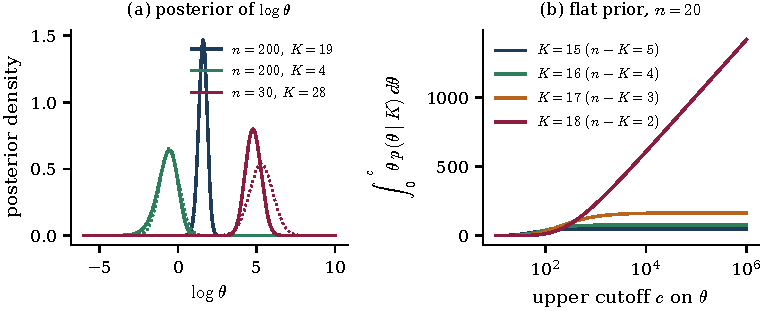
\includegraphics[width=\textwidth]{figures/pig_shape.pdf}
\caption{(a) Posterior of $\log\theta$ under a diffuse $\mathrm{Ga}(10^{-2},10^{-2})$ prior for three regimes; dotted curves are the Bernstein and von Mises Gaussians $\mathcal{N}(\log\hat\theta,J_n^{-1})$, accurate for moderate $K$ but not for small $K$ or $K\approx n$. (b) Under a flat prior with $n=20$, the posterior mean integral truncated at an increasing cutoff $c$ on $\theta$: finite and stable for $K\le n-4$, converging slowly at $K=n-3$, and divergent at $K=n-2$, as Proposition~\ref{pig:prop:tail} predicts.}
\label{pig:fig:shape}
\end{figure}

Under a genuinely flat prior the effect is sharper (Figure~\ref{pig:fig:shape}(b)). With $n=20$ the posterior mean is finite for $K\le n-3$, but at $K=n-2=18$ the truncated mean integral grows without bound as the cutoff is raised, taking values $111, 403, 748, 1101$ at $\theta\le e^6,e^8,e^{10},e^{12}$, an increase of about $175$ for every unit of $\log c$, which is the signature of a $\theta^{-2}$ tail: the posterior is proper yet has no finite mean. At $K=n-1$ it fails to integrate at all. A sample in which all but one or two specimens are distinct species carries almost no information from above about how much mass to hold in reserve for the unseen, and a flat prior does not supply the missing constraint.

\paragraph{A weakly informative PIG prior.} The remedy is a prior in the PIG family itself, specifically the $\tau=1$ case of the Diaconis and Ylvisaker prior~\eqref{pig:eq:conj} with $\kappa=K_0-1$: a single pseudosample
\begin{equation}\label{pig:eq:pigprior}
\pi(\theta)\propto\theta^{K_0-1}\frac{\Gamma(\theta)}{\Gamma(\theta+n_0)},
\end{equation}
read as ``in a pilot of $n_0$ specimens I saw $K_0$ species.'' Precisely, \eqref{pig:eq:pigprior} is the posterior that the scale invariant prior $\dd\theta/\theta$ would give after such a pilot sample. We take $(n_0,K_0)=(10,3)$, a prior with median $\theta\approx0.93$ carrying the weight of one small sample; it is proper because $0<K_0-1<n_0-1$. The posterior $p(\theta\mid K)\propto\theta^{K+K_0-1}[\Gamma(\theta)/\Gamma(\theta+n)][\Gamma(\theta)/\Gamma(\theta+n_0)]$ has tail $\theta^{K+K_0-1-n-n_0}$, so its mean and variance are finite for every $K\le n$; the pseudosample supplies exactly the upper tail information the data lack. It is sampled by the same augmentation with one extra latent, $\eta\sim\mathrm{Be}(\theta,n)$, $\eta_0\sim\mathrm{Be}(\theta,n_0)$, and $\theta\sim\mathrm{Ga}(K+K_0,\,-\log\eta-\log\eta_0)$. Being worth $K_0=3$ pseudospecies, it is negligible whenever the data are informative: for Williams it gives posterior mean $38.96$ (SD $2.79$) against the maximum likelihood value $40.15$, a shift of under half a posterior standard deviation. But it regularises the pathological cases. In the $n=30$, $K=28$ example the flat prior posterior mean is infinite and the diffuse $\mathrm{Ga}(10^{-2},10^{-2})$ gives 136 (an artefact of that prior's hidden exponential scale $1/b_0$), while the PIG prior returns a proper $40.7$ with a sensible interval $[17.3, 86.2]$. A diffuse gamma is not in fact noninformative for a parameter that may be large, since its rate fixes a scale; the PIG pseudosample regularises without imposing one.

These boundary regimes are what the posterior is for. The Beta augmentation sampler~\eqref{pig:eq:gibbs} stays valid throughout the proper range, since the conditional $\theta\mid\eta\sim\mathrm{Ga}(K+a_0,\,b_0-\log\eta)$ is a proper gamma draw with positive rate $b_0-\log\eta>0$ whatever the marginal tail, so the chain explores a skewed or infinite mean posterior without breaking and simply returns wide asymmetric intervals; when $K\ge n-1$ under a flat prior the chain instead drifts off to infinity, which is itself the signal that a proper prior is needed. Where Section~\ref{pig:sec:bvm} found the Bayes estimator of $\theta$ redundant, here it is the maximum likelihood point that misleads and the full posterior, with its skew and its honest tail, that is indispensable. The heavy tail is moreover native to the gamma ratio that the Beta block represents: its polynomial decay in $\theta$ drives Proposition~\ref{pig:prop:tail}, and the augmentation meets it without special treatment.

\paragraph{A real hyperdiverse sample.} Estimating how large a vocabulary an author commands is the unseen species problem in disguise, the reading \citet{pig:efron1976} gave the Shakespeare canon, and $n$ gram frequency smoothing remains the main modern home of the Good Turing estimator through the Katz backoff of language models. Taking a Shakespeare corpus of about $2\times10^5$ word tokens, the one parameter concentration behaves exactly as Proposition~\ref{pig:prop:tail} anticipates, and the choice of unit decides the regime. For word unigrams a sample of $n=500$ tokens contains $K=240$ types, $K/n=0.48$, and the likelihood is tight and nearly symmetric about the MLE 181: richness is well identified and the Bayes estimator sheds little, as in Section~\ref{pig:sec:bvm}. For word trigrams the same corpus is hyperdiverse. The first 50, 100, or 200 trigrams are all distinct, $K=n$, and the likelihood $\theta^K\Gamma(\theta)/\Gamma(\theta+n)$ tends to a nonzero constant as $\theta\to\infty$, since $\theta^n\Gamma(\theta)/\Gamma(\theta+n)\to1$: the maximum likelihood estimate is $+\infty$ and a flat prior posterior is improper (Figure~\ref{pig:fig:shakespeare}(b)). Here the weakly informative PIG prior does its work. Under the pseudosample prior $(n_0,K_0)=(10,3)$ the unigram posterior is barely moved (mean 170, skewness $0.28$, against MLE 181), while the trigram posteriors, improper under a flat prior when $K=n$, are proper: $n=100$ trigrams with $K=100$ give posterior mean 757 with interval $[331, 1649]$, and $n=400$, $K=396$ give mean 7700 with interval $[4100, 14100]$ (Figure~\ref{pig:fig:shakespeare}(a)). These posteriors are proper and finite but strongly prior influenced and enormous, the honest verdict that the data do not bound the concentration from above once almost every unit is a singleton.

\begin{figure}[t]
\centering
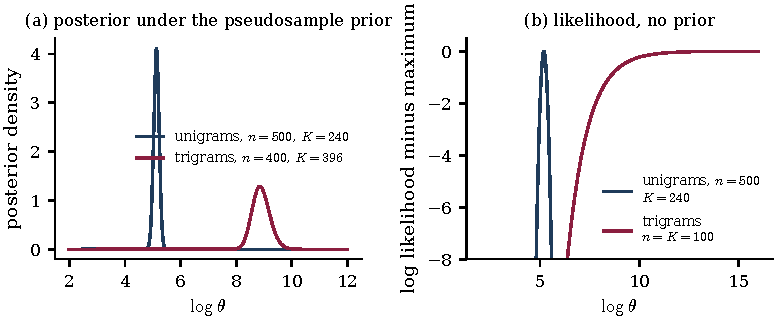
\includegraphics[width=\textwidth]{figures/pig_shakespeare.pdf}
\caption{Real hyperdiverse data: Shakespeare word units under the one parameter Ewens model. (a) Posterior of $\log\theta$ under the weakly informative PIG prior~\eqref{pig:eq:pigprior} with $(n_0,K_0)=(10,3)$; unigrams ($n=500$, $K=240$) give a tight symmetric posterior, trigrams ($n=400$, $K=396$) a proper but broad, prior regularised one near $\theta\approx7700$. (b) Log likelihood relative to its maximum, prior free; unigrams peak at $\hat\theta\approx181$, whereas trigrams with $K=n=100$ rise monotonically to a plateau, so $\theta$ has no finite maximiser and any flat prior posterior is improper.}
\label{pig:fig:shakespeare}
\end{figure}

Two lessons follow. First, the pathology is common, not exotic: any sparse categorical sample, $n$ grams, rare genetic variants, long tail catalogues, lands in it, and reporting an MLE or a symmetric interval for $\theta$ there would mislead badly where the honest posterior is heavy tailed or improper. In population genetic samples the same happens when nearly every sampled haplotype is unique, as in highly variable regions sequenced at modest depth. Second, near total distinctness is the fingerprint of a power law, which the one parameter Ewens model cannot represent; the second Pitman and Yor parameter $\sigma$ of~\eqref{pig:eq:py} absorbs it, trading an exploding $\theta$ for a finite pair $(\theta,\sigma)$ with $\sigma$ near one. The heavy tailed $\theta$ posterior is therefore also a specification diagnostic, and the PIG augmentation that samples it cleanly is what makes the diagnostic cheap to read.

\section{Fisher's two variances: a worked example}\label{pig:sec:twovariances}\sectionmark{Fisher's two variances}

This section works one example in detail and settles a point that confuses many readers of the classical literature: Fisher's unconditional model and Ewens' conditional model attach two different variances to the species count, and only one of them is the right yardstick for the uncertainty in $\theta$. We write $k$ for the observed number of species, as in the Dirichlet process literature. The concentration parameter governs partition diversity wherever exchangeable clustering arises. In population genetics, $\theta=4M\mu$ is the scaled mutation rate driving allele diversity \citep{pig:ewens1972}. In Bayesian nonparametrics, $\theta$ is the Dirichlet process concentration: $\E[K_n\mid\theta]\sim\theta\log n$, so misspecifying $\theta$ directly miscounts mixture components. In community ecology, $\theta$ is Fisher's diversity index, one of the oldest biodiversity statistics still in routine use \citep{pig:fisher1943}. In every case the parameter is weakly identified from a single partition and the likelihood is far from Gaussian.

\paragraph{The two variances.} In Fisher's model of Section~\ref{pig:sec:fisher} with $\nu=0$, the species count $K$ is a sum of independent Poisson multiplicities and is therefore itself Poisson, with variance equal to its mean, $\E[K]=\theta\log(1+\E[N]/\theta)$. This is the relation of \citet{pig:fisher1943}, and solving $K=\theta\log(1+N/\theta)$ for $\theta$ is Fisher's estimator. If one treats $K$ as Poisson with $N=n$ fixed and mean $m(\theta)=\theta\log(1+n/\theta)$, the delta method gives the Poisson variance
\begin{equation}\label{pig:eq:poisvar}
V_P(\theta)=\frac{m(\theta)}{m'(\theta)^2},\qquad m'(\theta)=\log\Bigl(1+\frac n\theta\Bigr)-\frac{n}{n+\theta}.
\end{equation}
In the Ewens model, by contrast, the sample size $n$ is fixed and the variance of $K$ is
\begin{equation}\label{pig:eq:esfvar}
\Var(K\mid\theta,n)=\sum_{j=0}^{n-1}\frac{\theta\,j}{(\theta+j)^2}=\theta[\psi(\theta+n)-\psi(\theta)]-\theta^2[\psi'(\theta)-\psi'(\theta+n)],
\end{equation}
as in Proposition~\ref{pig:prop:nef}, and the variance of the conditional MLE is $V_E(\theta)=\theta^2/\Var(K\mid\theta,n)=1/I(\theta)$. Both have the same form, (variance of $K$) divided by (slope of $\E[K]$ in $\theta$) squared; they differ in which variance of $K$ is used. For $1\ll\theta\ll n$ the expansions $\psi(\theta+n)-\psi(\theta)=\log(n/\theta)+O(1/\theta)$ and $\theta\psi'(\theta)=1+O(1/\theta)$ give
\[
\frac{\Var(K\mid\theta,n)}{\E[K\mid\theta,n]}\approx1-\frac{1}{\log(n/\theta)},\qquad V_E(\theta)\approx\frac{\theta}{\log(n/\theta)-1},
\]
whereas $V_P(\theta)\approx\theta\log(n/\theta)/\{\log(n/\theta)-1\}^2$. To leading order both are $\theta/\log(n/\theta)$, but the conditional variance is smaller by the factor $1-1/\log(n/\theta)$, which converges to one only logarithmically.

Which variance is right? Conditioning on $n$ removes the part of the variation in $K$ that is due to the random total $N$, and in Fisher's model $N$ carries almost no information about $\theta$: $N$ is negative binomial with shape $\theta$ and probability $x$, and once $x$ is profiled out the information about $\theta$ left in $N$ is about $1/(2\theta^2)$ (Exercise~\ref{pig:exr:ancillary}), against $I(\theta)\approx\{\log(n/\theta)-1\}/\theta$ in $K$ given $N$. For Williams that is $0.0003$ against $0.124$, a quarter of one percent. So $N$ is effectively ancillary for $\theta$, the conditional variance $V_E$ is the relevant one, and the Poisson variance overstates the standard error.

\begin{table}[t]
\centering
\caption{The two variances at the conditional MLE. $\E[K]$ and $\Var(K\mid n)$ from Proposition~\ref{pig:prop:nef}; SE (Ewens) $=V_E^{1/2}$ and SE (Poisson) $=V_P^{1/2}$ from~\eqref{pig:eq:poisvar}; the last column is Fisher's unconditional estimate from $K=\theta\log(1+n/\theta)$.}
\label{pig:tab:twovar}
\begin{adjustbox}{max width=\textwidth}
\begin{tabular}{@{}lrrrrrrr@{}}
\toprule
sample & $\hat\theta$ & $\E[K]$ & $\Var(K\mid n)$ & ratio & SE (Ewens) & SE (Poisson) & Fisher's $\tilde\theta$\\
\midrule
$n=200$, $k=25$ & 7.333 & 25.0 & 17.40 & 0.696 & 1.758 & 2.082 & 7.542\\
Williams 1933, $n=3540$, $k=178$ & 39.355 & 178.0 & 138.57 & 0.779 & 3.343 & 3.784 & 39.496\\
Williams, $n=15{,}609$, $k=240$ & 40.146 & 240.0 & 199.45 & 0.831 & 2.843 & 3.115 & 40.247\\
\bottomrule
\end{tabular}
\end{adjustbox}
\end{table}

Table~\ref{pig:tab:twovar} puts numbers on this. For the small sample the Poisson standard error is $18\%$ too large; for Williams it is $13\%$ too large in 1933 and $10\%$ too large for the full data. The approximation $V_E\approx\theta/\{\log(n/\theta)-1\}$ is excellent, giving the standard errors $1.783$, $3.354$ and $2.844$ against the exact $1.758$, $3.343$ and $2.843$, while the leading order $\theta/\log(n/\theta)$ gives $1.489$, $2.958$ and $2.595$, too small. Fisher's unconditional estimate for the full Williams data, $40.247$, matches the value $40.248$ quoted by \citet{pig:mccullagh2016}, and it differs from the conditional MLE by $0.1$, about $4\%$ of a standard error. Whichever estimator is used, the posterior of the next paragraphs is built on the exact conditional likelihood and so inherits the correct variance automatically; no choice between the two is needed.

\paragraph{Beta augmentation.} The likelihood of $K=k$ is $L(\theta\mid k)\propto\theta^k/(\theta)_{(n)}$, and the rising factorial in the denominator blocks conjugacy. Since $\Gamma(\theta)/\Gamma(\theta+n)=B(\theta,n)/\Gamma(n)$, the representation~\eqref{pig:eq:beta} introduces $\eta\in(0,1)$ as a latent and yields $p(\theta,\eta\mid k)\propto\pi(\theta)\,\theta^k\,\eta^{\theta-1}(1-\eta)^{n-1}$. With $\pi(\theta)=\mathrm{Ga}(a,b)$ the conditionals are those of~\eqref{pig:eq:gibbs} with $(K,a_0,b_0)=(k,a,b)$, a variant of the Escobar and West sampler \citep{pig:escobar1995}.

\paragraph{A heavy tailed prior.} For small $k$ the gamma prior in~\eqref{pig:eq:gibbs} leaks into the posterior through its rate. A natural heavy tailed alternative puts a half Cauchy prior on $\sqrt\theta$, the horseshoe choice for a scale parameter. If $\sqrt\theta\sim\mathrm{C}^+(0,1)$ then $\theta$ has the beta prime density $\pi(\theta)=\pi^{-1}\theta^{-1/2}(1+\theta)^{-1}$ and $\varphi=\log\theta$ has density $\{2\pi\cosh(\varphi/2)\}^{-1}$, a hyperbolic secant law. More generally the beta prime prior
\begin{equation}\label{pig:eq:betaprime}
\pi(\theta)\propto\theta^{\chi/2-1}(1+\theta)^{-\chi},\qquad\text{equivalently}\qquad p(\varphi)\propto\cosh^{-\chi}(\varphi/2),
\end{equation}
gives $\varphi$ a symmetric law with exponential tails of rate $\chi/2$. The P\'olya Gamma identity of \citet{pig:polson2013}, $\cosh^{-\chi}(\omega/2)=\E[e^{-\omega^2\Lambda/2}]$ with $\Lambda\sim\mathrm{PG}(\chi,0)$, writes this prior as a scale mixture of normals on $\log\theta$, but a Gaussian factor in $\log\theta$ does not combine conjugately with $\eta^\theta$. The gamma integral $(1+\theta)^{-\chi}=\Gamma(\chi)^{-1}\int_0^\infty\xi^{\chi-1}e^{-\xi(1+\theta)}\dd\xi$ does, and it gives a sampler in which every step is standard.

\begin{proposition}[Three block sampler]\label{pig:prop:threeblock}
Under the prior~\eqref{pig:eq:betaprime} the joint density
\[
p(\theta,\eta,\xi\mid k)\propto\theta^{k+\chi/2-1}\,\eta^{\theta-1}(1-\eta)^{n-1}\,\xi^{\chi-1}e^{-\xi(1+\theta)}
\]
on $(0,\infty)\times(0,1)\times(0,\infty)$ has $\theta$ marginal equal to the posterior $p(\theta\mid k)\propto\pi(\theta)\theta^k\Gamma(\theta)/\Gamma(\theta+n)$, and its full conditionals are
\begin{align*}
\eta\mid\theta&\sim\mathrm{Be}(\theta,n),\\
\xi\mid\theta&\sim\mathrm{Ga}(\chi,\,1+\theta),\\
\theta\mid\eta,\xi&\sim\mathrm{Ga}\bigl(k+\tfrac{\chi}{2},\,\xi-\log\eta\bigr).
\end{align*}
\end{proposition}

\begin{proof}
Integrating out $\eta$ with~\eqref{pig:eq:beta} produces $\Gamma(n)\Gamma(\theta)/\Gamma(\theta+n)$, and integrating out $\xi$ with the gamma integral produces $\Gamma(\chi)(1+\theta)^{-\chi}$, so the $\theta$ marginal is proportional to $\theta^{k+\chi/2-1}(1+\theta)^{-\chi}\Gamma(\theta)/\Gamma(\theta+n)$, which is the stated posterior. Each conditional is read off the joint density: in $\eta$ it is a $\mathrm{Be}(\theta,n)$ kernel; in $\xi$ it is $\xi^{\chi-1}e^{-\xi(1+\theta)}$; in $\theta$ it is $\theta^{k+\chi/2-1}e^{-\theta(\xi-\log\eta)}$, a gamma kernel with positive rate since $\xi>0$ and $\log\eta<0$.
\end{proof}

The half Cauchy case $\chi=1$ has $\theta$ shape $k+\tfrac12$, which is why the half integer appears. The tail of the posterior is $\theta^{k-n-\chi/2-1}$, so the prior adds $1+\chi/2$ powers of decay to the likelihood's $k-n$; with $\chi=1$ the posterior mean is finite whenever $k\le n-1$, two repeats better than the flat prior of Proposition~\ref{pig:prop:tail}.

\paragraph{Numerical example: \texorpdfstring{$n=200$, $k=25$}{n=200, k=25}.} Table~\ref{pig:tab:fisherbayes} and Figure~\ref{pig:fig:fisherbayes} compare Fisher's asymptotic answer with the posteriors under the diffuse gamma prior and under the half Cauchy prior on $\sqrt\theta$. The posterior summaries are by exact quadrature; the Beta augmentation sampler (200,000 draws) reproduces them to Monte Carlo error, with median $7.22$ and interval $[4.40, 11.32]$, and the three block sampler of Proposition~\ref{pig:prop:threeblock} gives median $7.10$ and interval $[4.32, 11.14]$ for the half Cauchy prior with integrated autocorrelation time $1.9$.

\begin{table}[t]
\centering
\caption{Fisher and Bayes for $n=200$, $k=25$. Spreads agree; shapes do not. Posterior summaries by exact quadrature. ``Right/left'' is $(q_{0.975}-\text{median})/(\text{median}-q_{0.025})$.}
\label{pig:tab:fisherbayes}
\small
\begin{tabular}{@{}lccc@{}}
\toprule
 & Fisher (asymptotic) & $\mathrm{Ga}(0.01,0.01)$ prior & half Cauchy on $\sqrt\theta$\\
\midrule
point estimate & $\hat\theta_{\mathrm{MLE}}=7.33$ & median $7.22$, mean $7.39$ & median $7.09$, mean $7.26$\\
spread & SE $=1.76$ & SD $=1.78$ & SD $=1.75$\\
95\% interval & $[3.89,\,10.78]$ & $[4.40,\,11.33]$ & $[4.31,\,11.15]$\\
skewness & $0$ (by construction) & $0.58$ & $0.58$\\
right/left & $1.00$ & $1.45$ & $1.46$\\
\bottomrule
\end{tabular}
\end{table}

\begin{figure}[t]
\centering
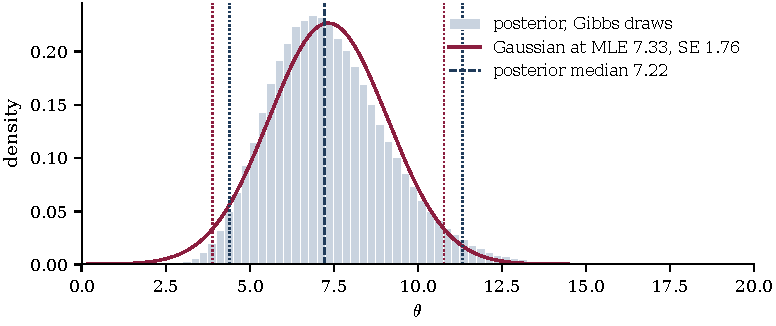
\includegraphics[width=\textwidth]{figures/pig_fisherbayes.pdf}
\caption{Posterior of $\theta$ for $n=200$, $k=25$ from the Beta augmentation sampler (histogram) overlaid with Fisher's information based Gaussian at the MLE (curve). Dotted lines mark the two $95\%$ intervals: the posterior interval $[4.40,11.32]$ and the Wald interval $[3.89,10.78]$. The posterior's right tail is about $45\%$ longer than its left.}
\label{pig:fig:fisherbayes}
\end{figure}

The summaries agree on the centre to within $0.3$ and on the spread to within $0.03$, yet disagree materially on coverage: Fisher's lower endpoint $3.89$ lies below the posterior $2.5\%$ quantile $4.40$, and Fisher's upper endpoint $10.78$ lies below the posterior $97.5\%$ quantile $11.33$. The entire Fisher interval is shifted left relative to the posterior because the Gaussian forces symmetry on a genuinely skewed object. The two priors differ by about $0.13$ in the centre, less than a tenth of a standard deviation, as Proposition~\ref{pig:prop:bvm} predicts for $k=25$.

\paragraph{Improvement over Fisher.} Fisher's interval treats the curvature at $\hat\theta$ as if it characterised the whole likelihood. In the Ewens problem it does not. The score is $k/\theta-\sum_{i<n}1/(\theta+i)\approx k/\theta-\log(n/\theta)$, so to the left of $\hat\theta$ the log likelihood plunges like $(k-1)\log\theta$ as $\theta\to0$, while to the right it declines only slowly, roughly linearly in $\theta$ while $\theta\ll n$ and eventually like $(k-n)\log\theta$. The right tail is therefore longer and the posterior is right skewed whenever $k\ll n$. Three concrete improvements follow.

\emph{(i) Honest coverage.} The Bayesian interval is asymmetric by construction and reproduces the true tail behaviour (Figure~\ref{pig:fig:fisherbayes}); Fisher's symmetric interval puts too much probability on the left and too little on the right.

\emph{(ii) Robustness in the data poor regime.} When $k$ is small the gamma prior's rate and shape both matter. At $n=200$, $k=3$ the diffuse gamma prior gives posterior mean $0.38$ and interval $[0.045, 1.11]$, the half Cauchy prior $0.43$ and $[0.067, 1.16]$; the heavy tailed prior keeps the lower endpoint from being dragged toward zero by the gamma shape $a_0=0.01$. At the other boundary, $n=30$, $k=28$, the half Cauchy prior gives a posterior median of $175$ and interval $[54, 958]$ with a finite mean but an infinite third moment, honestly reporting how little the data say; the three block sampler then mixes slowly (integrated autocorrelation time about $30$ to $35$), a computational echo of the heavy tail. The weakly informative PIG prior of Section~\ref{pig:sec:tails} is the better choice there.

\emph{(iii) One variance instead of two.} The posterior is built from the exact conditional likelihood, so its spread is automatically governed by $\Var(K\mid\theta,n)$ and not by the Poisson variance~\eqref{pig:eq:poisvar}; Table~\ref{pig:tab:fisherbayes} shows the posterior SD $1.78$ agreeing with the Ewens SE $1.76$ and not with the Poisson SE $2.08$. The construction is closed form Gibbs throughout.

\section{Numerical study}\label{pig:sec:numerical}

This section collects the simulation checks behind the claims of the chapter and completes the analysis of Williams' Rothamsted Macrolepidoptera. Unless stated otherwise the prior is the diffuse $\mathrm{Ga}(10^{-2},10^{-2})$ and every chain uses the stable Beta draw of Remark~\ref{pig:rem:smallbeta}.

\paragraph{Good's rule (Table~\ref{pig:tab:good}, Figure~\ref{pig:fig:goodturing}(a)).} Monte Carlo expected multiplicities from the Chinese restaurant process match the closed form of Proposition~\ref{pig:prop:good}, and Good's estimator~\eqref{pig:eq:good} evaluated with the exact $\mu_{r,n}$ reproduces $r/(n+\theta)$ to rounding error, as an identity must.

\begin{table}[t]
\centering
\caption{Good Turing reconciliation, $\theta=3$, $n=40$. Monte Carlo $\E[a_r]$ ($6\times10^4$ simulated partitions) against the closed form, and Good's estimator with exact $\mu_{r,n}$ against $r/(n+\theta)$.}
\label{pig:tab:good}
\small
\begin{tabular}{@{}ccccc@{}}
\toprule
$r$ & $\E[a_r]$ Monte Carlo & $\E[a_r]$ formula & Good's \eqref{pig:eq:good} & $r/(n+\theta)$\\
\midrule
1 & 2.858 & 2.857 & 0.02326 & 0.02326\\
2 & 1.361 & 1.359 & 0.04651 & 0.04651\\
3 & 0.863 & 0.861 & 0.06977 & 0.06977\\
4 & 0.616 & 0.612 & 0.09302 & 0.09302\\
5 & 0.460 & 0.464 & 0.11628 & 0.11628\\
6 & 0.368 & 0.366 & 0.13953 & 0.13953\\
\bottomrule
\end{tabular}
\end{table}

\paragraph{Posteriors reproduce the likelihood (Figure~\ref{pig:fig:posterior}).} With $\theta=5$ and $n=1000$ the expected species count is $\E[K\mid\theta]=27.03$, and we condition on the typical value $K=27$. The diffuse prior posterior mean is then $5.01$ (SD $1.08$) against MLE $4.99$ (SE $1.08$). For Williams ($n=15{,}609$, $K=240$) the conditional MLE is $\hat\theta=40.146$ (SE $2.843$), matching \citet{pig:mccullagh2016} to three decimals; the posterior mean is $40.09$ (SD $2.84$), with Fisher's unconditional $40.248$ marked for comparison.

\begin{figure}[t]
\centering
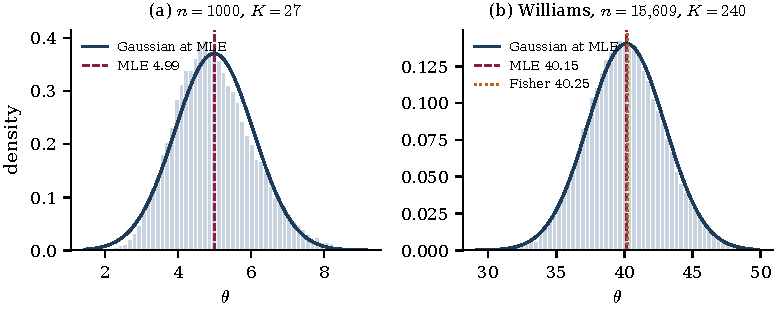
\includegraphics[width=\textwidth]{figures/pig_posterior.pdf}
\caption{Posterior of $\theta$ (histogram of $40{,}000$ Beta augmentation draws) against the Gaussian centred at the MLE with the asymptotic standard error (Proposition~\ref{pig:prop:bvm}). (a) $n=1000$, $K=27$, the expected species count when $\theta=5$. (b) Williams' Macrolepidoptera, $n=15{,}609$, $K=240$. In both the Bayes point estimate and interval reproduce the likelihood.}
\label{pig:fig:posterior}
\end{figure}

\paragraph{Computation and prior sensitivity (Table~\ref{pig:tab:sampler}, Figure~\ref{pig:fig:mixing}).} The Beta augmentation sampler~\eqref{pig:eq:gibbs} is nearly i.i.d.\ (integrated autocorrelation time $1.4$) and delivers about seven times the effective samples per second of a random walk Metropolis sampler on $\log\theta$ with proposal standard deviation $0.07$, whose chain has autocorrelation time $8.9$. That proposal is narrower than optimal: at the best scale, standard deviation about $0.17$ with acceptance rate $0.44$, the autocorrelation time is about $4.4$, which roughly halves the advantage. The timings are for plain Python loops and only their ratio is meaningful. Across 150 simulated data sets with $\theta=6$, $n=800$ the posterior mean exceeds the MLE by $0.019$ on average and never by more than $0.02$, under two percent of a standard error. A coverage experiment with the same design and 400 data sets (mean $K=30.1$) gives $92.8\%$ empirical coverage of the nominal $95\%$ credible interval, $91.3\%$ for the Wald interval and $93.3\%$ for the log scale Wald interval; with 400 replications the Monte Carlo standard error is about $1.3$ points, and the shortfall reflects the moderate information at $K\approx30$ and the discreteness of $K$.

\begin{table}[t]
\centering
\caption{Sampler efficiency for the Williams posterior ($n=15{,}609$, $K=240$), 16,000 retained draws. The exact posterior mean and SD are $40.088$ and $2.838$. IAT is the integrated autocorrelation time, ESS the effective sample size; ESS per second is for plain Python loops on one core.}
\label{pig:tab:sampler}
\footnotesize
\setlength{\tabcolsep}{3pt}
\begin{tabular}{@{}lrrrrrc@{}}
\toprule
sampler & mean & SD & IAT & ESS & ESS/sec & acc.\\
\midrule
PIG Beta augmentation \eqref{pig:eq:gibbs} & 40.127 & 2.860 & 1.40 & 11,410 & 147,600 & n/a\\
random walk Metropolis & 40.056 & 2.871 & 8.92 & 1,794 & 20,571 & 0.71\\
\bottomrule
\end{tabular}
\end{table}

\begin{figure}[t]
\centering
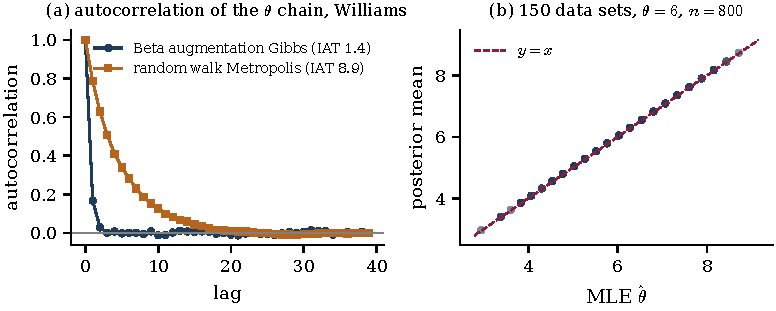
\includegraphics[width=\textwidth]{figures/pig_mixing.pdf}
\caption{(a) Autocorrelation of the $\theta$ chain for the Williams posterior: the PIG Beta augmentation sampler decorrelates in one or two steps, random walk Metropolis in about ten. (b) Posterior mean against MLE over 150 data sets ($\theta=6$, $n=800$); the estimators are interchangeable.}
\label{pig:fig:mixing}
\end{figure}

\paragraph{Prior sensitivity.} Proposition~\ref{pig:prop:bvm} concerns priors flat near $\hat\theta$, and among these the Williams posterior is stable: the diffuse $\mathrm{Ga}(10^{-3},10^{-3})$ gives posterior mean $40.16$, the default $\mathrm{Ga}(10^{-2},10^{-2})$ gives $40.09$, and a $\mathrm{Ga}(2,0.05)$ prior with mean 40 gives $40.16$, all within $0.03$ posterior standard deviations of each other. The claim is not that no prior can matter at finite $K$. An aggressive $\mathrm{Ga}(1,1)$, effectively $\mathrm{Exp}(1)$ favouring small $\theta$, pulls the mean to $33.69$, a $16\%$ shift, because its rate $1$ competes with the modest data rate $\E[-\log\eta]=\psi(\theta+n)-\psi(\theta)\approx\log\{(n+\theta)/\theta\}\approx6$ in the gamma step of~\eqref{pig:eq:gibbs}. With effective sample size $K=240$ the likelihood dominates any diffuse prior but not an informative one, exactly as the logarithmic information growth predicts.

\paragraph{The PIG(0) engine and Fisher's \texorpdfstring{$\nu$}{nu} (Table~\ref{pig:tab:pig0}, Figure~\ref{pig:fig:pig0}).} Simulating $X_0$ by the inverse gamma series of Proposition~\ref{pig:prop:pig0}, truncated at $1500$ terms with the mean of the remainder, $\sum_{k>1500}1/(2k^2)=3.3\times10^{-4}$, added as a constant, and comparing $\widehat{\E}[e^{-s^2X_0}]$ over $2\times10^5$ draws to the exact reciprocal gamma transform $e^{-\gamma s}/\Gamma(1+s)$ gives agreement within $0.07\%$ over $s\in[0.25,2]$. The sample mean is $0.801$ against $\pi^2/12=0.822$; the gap is not an error but a consequence of $\Var(X_0)=\infty$, which makes the sample mean converge slowly and erratically, and it is why the Laplace transform, a bounded function of $X_0$, is the right check. For Fisher's $\nu$ we simulated $400$ species abundances from the zero truncated negative binomial of~\eqref{pig:eq:nbseries} with $x=0.98$ and computed the joint posterior of $(\nu,x)$ under flat priors on $\nu\in(0,1.2]$ and $x\in[0.9,1)$ by quadrature, which is the target that the R2 Gibbs sampler draws from. Log series data (true $\nu=0$, $5568$ specimens) yield posterior mean $0.027$ with $95\%$ interval $[0, 0.075]$, recovering Fisher's empirical conclusion, while $\nu=0.5$ data ($11{,}886$ specimens) are recovered at $0.55$ with interval $[0.43, 0.67]$.

\begin{table}[t]
\centering
\caption{PIG(0) simulator ($2\times10^5$ draws, 1500 term truncation plus remainder mean) against the exact reciprocal gamma transform~\eqref{pig:eq:pig0}.}
\label{pig:tab:pig0}
\small
\begin{tabular}{@{}cccc@{}}
\toprule
$s$ & $\widehat{\E}[e^{-s^2X_0}]$ & $e^{-\gamma s}/\Gamma(1+s)$ & rel.\ error\\
\midrule
0.25 & 0.95532 & 0.95501 & $3.3\times10^{-4}$\\
0.50 & 0.84603 & 0.84550 & $6.2\times10^{-4}$\\
1.00 & 0.56177 & 0.56146 & $5.5\times10^{-4}$\\
1.50 & 0.31651 & 0.31648 & $0.9\times10^{-4}$\\
2.00 & 0.15756 & 0.15762 & $3.9\times10^{-4}$\\
\bottomrule
\end{tabular}
\end{table}

\begin{figure}[t]
\centering
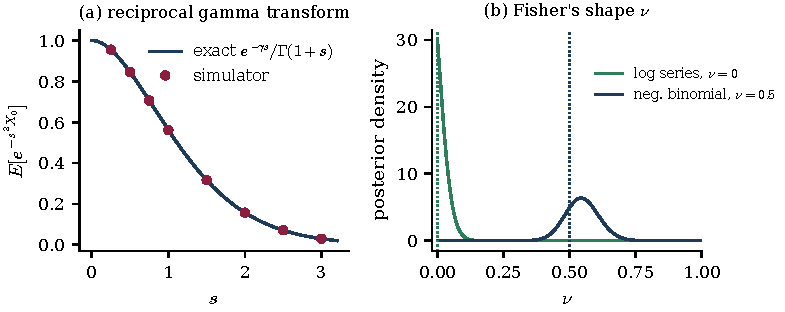
\includegraphics[width=\textwidth]{figures/pig_pig0.pdf}
\caption{(a) The PIG(0) simulator (points) reproduces the exact reciprocal gamma transform $e^{-\gamma s}/\Gamma(1+s)$ (curve). (b) Posterior of Fisher's shape $\nu$ from 400 simulated species: log series data concentrate at $\nu=0$ (the Ewens limit), and $\nu=0.5$ data are recovered.}
\label{pig:fig:pig0}
\end{figure}

\paragraph{Good Turing for Williams (Figure~\ref{pig:fig:goodturing}(b)).} Pushing the posterior draws through $r/(n+\theta)$ gives Bayesian Good Turing frequencies. For the seen species the posterior is degenerate for practical purposes: $q_1$ has posterior mean $6.390\times10^{-5}$ with $95\%$ interval $[6.388, 6.392]\times10^{-5}$, a relative width of $0.07\%$, slightly below the raw proportion $1/n=6.407\times10^{-5}$ because of the shrinkage factor $n/(n+\theta)=0.9974$. The unseen mass is where the posterior matters: $q_0=\theta/(n+\theta)$ has posterior mean $2.56$ per thousand with interval $[2.22, 2.92]$ per thousand, a relative width of $27\%$.

\begin{figure}[t]
\centering
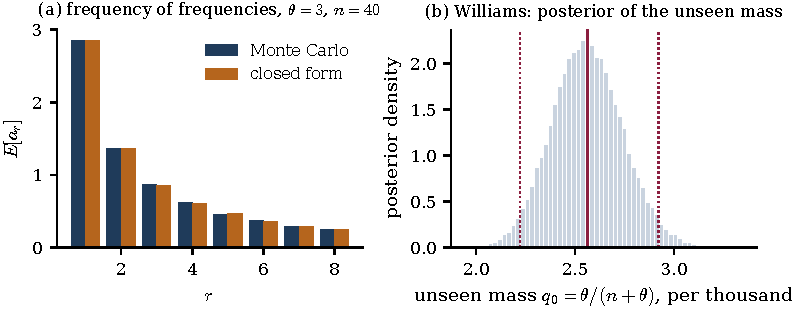
\includegraphics[width=\textwidth]{figures/pig_goodturing.pdf}
\caption{(a) Expected frequency of frequencies for $\theta=3$, $n=40$: Monte Carlo against the closed form of Proposition~\ref{pig:prop:good}. (b) Posterior of the unseen mass $q_0=\theta/(n+\theta)$ for Williams, in units of one per thousand; the solid line is the posterior mean and the dotted lines the $95\%$ interval. The corresponding bands for the seen frequencies $q_r=r/(n+\theta)$, $r\ge1$, have relative width below $0.1\%$ and are not shown.}
\label{pig:fig:goodturing}
\end{figure}

\paragraph{Williams temporal homogeneity (Figure~\ref{pig:fig:predictive}).} Refitting the year 1933 alone ($n=3540$, $K=178$) gives $\hat\theta=39.355$, exactly \citet{pig:mccullagh2016}, with posterior mean $39.3$ (SD $3.3$). For the 12,069 specimens of 1934 to 1936, Proposition~\ref{pig:prop:newspecies} gives the expected number of new species, $\E[U_m\mid\theta]$, which has posterior mean $58.0$ with $95\%$ interval $[48.8, 68.0]$, reproducing McCullagh's plug in value $58.06$. The full predictive distribution of the count itself, computed exactly by mixing the Poisson binomial law of $U_m$ over the posterior of $\theta$, has mean $58.0$ and standard deviation $9.0$, of which the sampling term contributes variance $57.6$ and the parameter term $24.0$; its $95\%$ interval is $[41, 77]$ and the probability of $62$ or more new species is $0.34$. The observed 62 is well inside both intervals: no evidence against temporal homogeneity, now with a calibrated interval rather than a point.

The full \citet{pig:goodtoulmin1956} accumulation curve, obtained by propagating the same posterior through the predictive law for every $m$, is shown in Figure~\ref{pig:fig:accumulation}. The $95\%$ predictive band is $[9, 27]$ at $m=2000$, $[26, 53]$ at $m=6000$ and $[41, 76]$ at $m=12{,}000$; the observed count lies inside the band, and the band widens without ever narrowing, the honest reflection of the logarithmic information in $K$: extrapolation is possible but its uncertainty never collapses. This curve, with its interval, is the deliverable Good and Toulmin were reaching for and the Bayesian object that the richness point estimate cannot provide.

\begin{figure}[t]
\centering
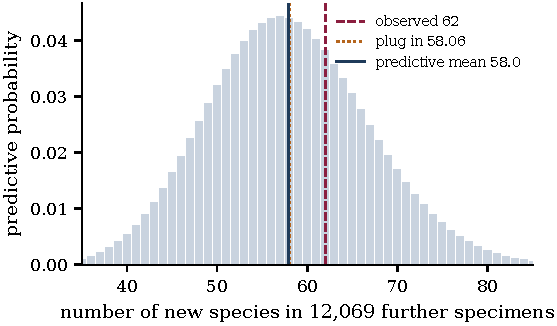
\includegraphics[width=0.75\textwidth]{figures/pig_predictive.pdf}
\caption{Posterior predictive distribution of the number of new species among 12,069 further specimens under the Ewens process fitted to 1933, including both sampling and parameter uncertainty. The observed 62 and McCullagh's plug in 58.06 both fall in the bulk.}
\label{pig:fig:predictive}
\end{figure}

\begin{figure}[t]
\centering
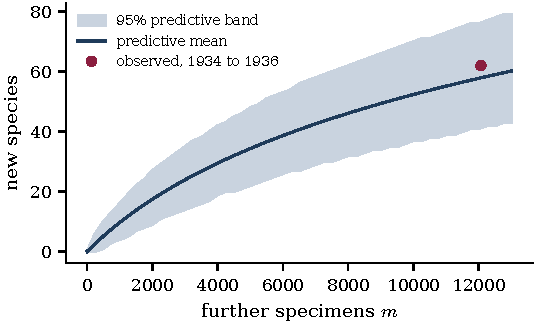
\includegraphics[width=0.75\textwidth]{figures/pig_accumulation.pdf}
\caption{Posterior predictive species accumulation curve (Good and Toulmin) from the 1933 fit: predictive mean and $95\%$ predictive band for the number of new species among $m$ further specimens. The observed 62 new species at $m=12{,}069$ falls within the band.}
\label{pig:fig:accumulation}
\end{figure}

\section{Discussion}\label{pig:sec:discussion}

The Fisher and Ewens richness problem is the cleanest instance of a division of labour that recurs whenever a model reduces to a low dimensional sufficient statistic in a regular exponential family. For estimating $\theta$ the Bayes rule is a reparametrised maximum likelihood estimate and the prior is a rounding error, a fact Proposition~\ref{pig:prop:bvm} makes quantitative through the effective sample size $K$. The genuinely Bayesian content lies elsewhere, in the predictive law the model induces: the Chinese restaurant rule $r/(n+\theta)$, its unseen mass specialisation $\theta/(n+\theta)$, and the Good and Toulmin accumulation curve, each carried with an honest posterior band. This is the de Finetti reading of \citet{pig:goodtoulmin1956}: had they grafted a parametric skeleton onto their sequential prediction, the exchangeable partition process would have appeared, and Proposition~\ref{pig:prop:good} shows their own estimator was already that process in disguise.

P\'olya inverse gamma augmentation is the computational thread that ties the three classical viewpoints together. Its two representations answer to Fisher's two parameters: the gamma ratio for richness, where inference is easy and the Bayesian gain is slight, and the reciprocal gamma for the shape $\nu$, where inference is genuinely hard and the PIG engine earns its place. Beneath both sits the gamma subordinator, the prototypical generalized gamma convolution, whose normalisation is Ferguson's Dirichlet process and whose sample partition is Kingman's Ewens formula, and whose discretised L\'evy density is Fisher's log series. Read this way, Fisher's estimation, Good's smoothing, and PIG augmentation are three views of one gamma process structure, and the division of labour between what the Bayes estimator can and cannot add follows from where in that structure information accumulates: logarithmically for $\theta$, and not at all from above once the sample is saturated with singletons.

That last qualification is the second half of the chapter and it tempers the first. ``Sheds little'' is a statement about the interior of the range $1<K<n$. At the boundaries the posterior for the concentration is strongly skewed, and heavy tailed when $K$ is near $n$, and the roles reverse: for a hyperdiverse sample it is the maximum likelihood point that misleads, running off to infinity when every unit is distinct, while the full posterior with its honest tail is indispensable. A flat prior is not merely vague there but improper, and a diffuse gamma is not innocent either, since its rate quietly fixes a scale. Our recommendation is the weakly informative PIG prior~\eqref{pig:eq:pigprior}, a single pseudosample in the same gamma ratio family, which guarantees a proper posterior with finite mean and variance for every $K\le n$, costs one extra Beta draw, and is dominated by any informative sample. It also serves as a specification diagnostic: an exploding concentration under this prior is the fingerprint of a power law that the one parameter model cannot represent, and it points directly to the second parameter that can.

Several limitations bound the claims and mark the natural next steps. The one parameter Ewens model is misspecified for power law data, and the honest response is the two parameter Pitman and Yor process of~\eqref{pig:eq:py}, whose discount $\sigma$ absorbs the heavy tail; we placed it in the family but did not fit it, so the Shakespeare trigram posteriors should be read as diagnostics rather than estimates. Our recovery of Fisher's shape $\nu$ used simulated frequencies because the Williams analysis here uses only the pair $(n,K)$ for each period, so a full two parameter fit to primary frequency data through the reciprocal gamma augmentation R2 remains open; the butterfly example of Section~\ref{pig:sec:good} shows that even fifteen cells of a frequency table identify the log series richness well, though not its second parameter $x$. The Bernstein and von Mises statement is asymptotic in $K$, and at the moderate values typical of ecological samples the Gaussian approximation is only approximate, as the $93\%$ interval coverage at $K\approx30$ records. None of these caveats disturbs the reconciliations, which are exact identities, but each marks where the modelling, as opposed to the mathematics, must be taken further.

The structure generalises beyond the scalar problem. The reciprocal gamma representation R2 handles the vector concentration of the finite Dirichlet multinomial and the shape of a gamma mixing measure, so the same augmentation supports species models with covariates and hierarchical concentrations shared across sites or years, all within one gamma and Beta sampler. More broadly, placing Fisher, Good, and Ewens inside the generalized gamma convolution class connects a classical problem to the wider PIG program and to the Thorin measure calculus that indexes it. On the applied side, the Good Turing rule remains the workhorse of $n$ gram smoothing in language models, and a Bayesian version that reports the unseen mass with a calibrated interval, rather than a point, may be useful wherever that mass carries decision weight, from estimating undetected biodiversity to sizing a vocabulary to bounding the burden of rare genetic variants.

\section{Proofs}\label{pig:sec:proofs}

\begin{proof}[Proof of Proposition~\ref{pig:prop:nef}]
From~\eqref{pig:eq:esf}, $p(a\mid\theta)=h(a)\,\theta^K/(\theta)_{(n)}$ with $h(a)=n!\prod_j(j^{a_j}a_j!)^{-1}$. Writing $\varphi=\log\theta$ gives $p=h(a)\exp\{\varphi K-A(\varphi)\}$ with $A(\varphi)=\log(\theta)_{(n)}=\log\Gamma(\theta+n)-\log\Gamma(\theta)$. The natural parameter space is all of $\mathbb{R}$, which is open, so the family is regular. Then $\mathrm{d}A/\mathrm{d}\varphi=(\mathrm{d}A/\mathrm{d}\theta)\theta=\theta[\psi(\theta+n)-\psi(\theta)]$. For the Feller coupling, run the Chinese restaurant process and let $B_i$ indicate that the specimen arriving when $i$ are present founds a new species; it does so with probability $\theta/(\theta+i)$ whatever the earlier configuration, so the $B_i$ are independent and $K=\sum_{i=0}^{n-1}B_i$. Hence $\E[K]=\sum_i\theta/(\theta+i)$, which equals $\theta[\psi(\theta+n)-\psi(\theta)]$ by the recurrence $\psi(x+1)=\psi(x)+1/x$, and this is $A'(\varphi)$ as the exponential family identity requires. Likewise $\Var(K)=\sum_i\frac{\theta}{\theta+i}\cdot\frac{i}{\theta+i}=\sum_i\theta i/(\theta+i)^2$; differentiating $A'(\varphi)=\sum_i e^\varphi/(e^\varphi+i)$ once more gives the same sum, so $A''(\varphi)=\Var(K)$, positive as soon as $n\ge2$. Convexity of $A$ gives strict concavity of the log likelihood $\varphi K-A(\varphi)$ and uniqueness of the root of~\eqref{pig:eq:moment}, which exists when $1<K<n$ because $A'$ increases from $1$ to $n$. Finally
\[
I(\theta)=A''(\varphi)\Bigl(\frac{\mathrm{d}\varphi}{\mathrm{d}\theta}\Bigr)^2=\frac{\Var(K)}{\theta^2},
\]
and expanding, $I(\theta)=\theta^{-1}\sum_i i/(\theta+i)^2$.
\end{proof}

\begin{proof}[Propriety of~\eqref{pig:eq:conj}]
As $\theta\to0^+$, $\Gamma(\theta)/\Gamma(\theta+n_0)\sim1/(\theta\,\Gamma(n_0))$, so the integrand behaves like $\theta^{\kappa-\tau}$, integrable near zero if and only if $\kappa-\tau>-1$. As $\theta\to\infty$, $\Gamma(\theta)/\Gamma(\theta+n_0)\sim\theta^{-n_0}$, so the integrand behaves like $\theta^{\kappa-\tau n_0}$, integrable at infinity if and only if $\kappa-\tau n_0<-1$. The integrand is continuous and positive in between. Both conditions hold for some $\kappa$ precisely when $\tau-1<\tau n_0-1$, that is $n_0>1$.
\end{proof}

\begin{proof}[Proof of Proposition~\ref{pig:prop:pig0}]
For $Y\sim\mathrm{InvGa}(3/2,1)$ and $t>0$, substituting $y=1/u$,
\[
\E[e^{-tY}]=\frac{1}{\Gamma(3/2)}\int_0^\infty u^{1/2}e^{-u-t/u}\dd u=(1+2\sqrt t)\,e^{-2\sqrt t},
\]
by the standard integral $\int_0^\infty u^{1/2}e^{-u-t/u}\dd u=\tfrac{\sqrt\pi}{2}(1+2\sqrt t)e^{-2\sqrt t}$. With $t=s^2/(4k^2)$ this is $(1+s/k)e^{-s/k}$. The terms $Y_k/(4k^2)$ are independent and nonnegative with $\sum_k\E[Y_k]/(4k^2)=\sum_k 1/(2k^2)<\infty$, since $\E[Y]=1/(3/2-1)=2$; so the series converges almost surely and in mean, and by monotone convergence
\[
\E[e^{-s^2X_0}]=\prod_{k\ge1}\Bigl(1+\frac sk\Bigr)e^{-s/k}=\frac{e^{-\gamma s}}{\Gamma(1+s)},
\]
the last step being the Weierstrass product $1/\Gamma(1+s)=e^{\gamma s}\prod_k(1+s/k)e^{-s/k}$. The mean is $\sum_k 2/(4k^2)=\zeta(2)/2=\pi^2/12$. Finally $\E[Y^2]=\infty$ because the $\mathrm{InvGa}(3/2,1)$ density decays like $y^{-5/2}$, and since $X_0\ge Y_1/4$ we have $\E[X_0^2]=\infty$. As a cross check on the mean, $\log\E[e^{-s^2X_0}]=-\gamma s-\log\Gamma(1+s)=-\sum_{k\ge2}(-1)^k\zeta(k)s^k/k$, so $\E[e^{-s^2X_0}]=1-\tfrac12\zeta(2)s^2+O(s^3)$; the presence of an $s^3$ term, odd in $s$, is another sign that $X_0$ has no second moment.
\end{proof}

\begin{proof}[Proof of Proposition~\ref{pig:prop:good}]
By exchangeability, label the specimens $1,\dots,n$; then
\[
\E[a_r(n)]=\binom{n}{r}\Pr(\text{a fixed set } S \text{ of } r \text{ specimens is exactly one block}),
\]
and since the law is exchangeable we may take $S=\{1,\dots,r\}$, the first $r$ arrivals. Under the Chinese restaurant process the first arrival opens a block, and the arrival that finds $i$ specimens all in that block joins it with probability $i/(\theta+i)$, so the first $r$ form one block with probability $\prod_{i=1}^{r-1}i/(\theta+i)=(r-1)!\,\Gamma(\theta+1)/\Gamma(\theta+r)$. Each of the remaining arrivals, finding $r+j$ specimens present ($j=0,\dots,n-r-1$), avoids that block of size $r$ with probability $(\theta+j)/(\theta+r+j)$, whatever happens elsewhere. The product of these is $\frac{\Gamma(\theta+n-r)}{\Gamma(\theta)}\cdot\frac{\Gamma(\theta+r)}{\Gamma(\theta+n)}$, and multiplying the two factors gives $\theta(r-1)!\,\Gamma(\theta+n-r)/\Gamma(\theta+n)$ for the probability that $S$ is a block. Multiplying by $\binom nr$,
\[
\E[a_r(n)]=\frac{\theta}{r}\,\frac{n!}{(n-r)!}\,\frac{\Gamma(\theta+n-r)}{\Gamma(\theta+n)},
\]
which at $r=n$ reduces to $\theta\Gamma(n)\Gamma(\theta)/\Gamma(\theta+n)$, the probability of a single block. Substituting $\mu_{r,n}$ and $\mu_{r+1,n+1}$ into~\eqref{pig:eq:good}, the factors $\Gamma(\theta+n-r)$ cancel and
\[
\frac{\mu_{r+1,n+1}}{\mu_{r,n}}=\frac{r}{r+1}\,(n+1)\,\frac{\Gamma(\theta+n)}{\Gamma(\theta+n+1)}=\frac{r}{r+1}\,\frac{n+1}{\theta+n},
\]
so $\E[q_r\mid\text{data}]=\frac{r+1}{n+1}\cdot\frac{r}{r+1}\cdot\frac{n+1}{\theta+n}=\frac{r}{n+\theta}$. The unseen mass $q_0=\theta/(n+\theta)$ is the Chinese restaurant probability of opening a new block, and the masses add up correctly: $\sum_r a_r\,r/(n+\theta)+\theta/(n+\theta)=(n+\theta)/(n+\theta)=1$.
\end{proof}

\begin{proof}[Proof of Proposition~\ref{pig:prop:newspecies}]
Continue the Chinese restaurant process past $n$. The arrival that finds $i\ge n$ specimens present founds a new species with probability $\theta/(\theta+i)$, independently of the configuration and hence of the first $n$ specimens, and every species founded after time $n$ is new relative to the sample. So $U_m=\sum_{i=n}^{n+m-1}B_i$ with independent Bernoulli $B_i$, and the mean and variance follow as in the proof of Proposition~\ref{pig:prop:nef}, using $\sum_{i=n}^{n+m-1}1/(\theta+i)=\psi(\theta+n+m)-\psi(\theta+n)$. Given the data, $U_m$ depends on the sample only through $\theta$, whose posterior depends only on $K$; the law of total variance then gives the stated decomposition.
\end{proof}

\begin{proof}[Proof of Proposition~\ref{pig:prop:bvm}]
This is Bernstein and von Mises for a regular one parameter NEF \citep[Chapter 10]{pig:vandervaart1998}, with $J_n=A''(\hat\varphi)\to\infty$ playing the role of the sample size: the log likelihood $\varphi K-A(\varphi)$ is concave with curvature $A''$, and $A'''(\varphi)/A''(\varphi)^{3/2}\to0$ as $J_n\to\infty$ because the cumulants of the sum of independent Bernoulli variables $K$ are all of order $\E[K]$. Hence the posterior of $\varphi$ converges in total variation to $\mathcal{N}(\hat\varphi,J_n^{-1})$. A Laplace expansion of $\E[e^\varphi\mid K]$ about $\hat\varphi$ gives $\E[\theta\mid K]=\hat\theta\{1+O(J_n^{-1})\}$, and the delta method maps the Gaussian interval for $\varphi$ to the Wald interval for $\theta$ with error $o(\hat\theta J_n^{-1/2})$. Reweighting the prior by a smooth positive $g$ shifts the posterior mean of $\varphi$ by $J_n^{-1}(\log g)'(\hat\varphi)+o(J_n^{-1})$, hence the posterior mean of $\theta$ by
\[
\hat\theta\,J_n^{-1}(\log g)'(\hat\varphi)+o(\hat\theta J_n^{-1}),
\]
and changes the posterior by $O(J_n^{-1/2})$ in total variation. Since $J_n$ is of the order of $\E[K]$, the effective sample size is $K$.
\end{proof}

\begin{proof}[Proof of Proposition~\ref{pig:prop:tail}]
Since $\Gamma(\theta)/\Gamma(\theta+n)=\prod_{i=0}^{n-1}(\theta+i)^{-1}$ and each factor is asymptotic to $\theta^{-1}$, the ratio is $\sim\theta^{-n}$ as $\theta\to\infty$, so the posterior integrand satisfies
\[
\theta^{K+a_0-1}e^{-b_0\theta}\,\frac{\Gamma(\theta)}{\Gamma(\theta+n)}\sim\theta^{K+a_0-1-n}e^{-b_0\theta}.
\]
If $b_0>0$ the exponential dominates and every moment is finite. If $b_0=0$ the tail is $\theta^{K+a_0-1-n}$; $\int^\infty\theta^{K+a_0-1-n}\dd\theta<\infty$ if and only if $K+a_0-1-n<-1$, that is $K+a_0<n$, and $\int^\infty\theta^p\theta^{K+a_0-1-n}\dd\theta<\infty$ if and only if $p<n-K-a_0$. Integrability at $\theta\to0^+$ holds throughout since $\Gamma(\theta)/\Gamma(\theta+n)\sim1/(\theta\Gamma(n))$ makes the integrand $O(\theta^{K+a_0-2})$ with $K+a_0-2>-1$ for $K\ge1$. Substituting $(a_0,b_0)=(1,0)$ gives propriety for $K<n-1$, finite mean for $K<n-2$, and finite variance ($p=2$) for $K<n-3$, that is $K\le n-2,\ n-3,\ n-4$ respectively.
\end{proof}

\section{Sampler details}\label{pig:sec:sampler}

\emph{Richness $\theta$.} Prior $\mathrm{Ga}(a_0,b_0)$; iterate~\eqref{pig:eq:gibbs}, drawing $\log\eta$ as in Remark~\ref{pig:rem:smallbeta}, and replacing the single Beta by one draw per sample for multiyear data, in which case the gamma rate is $b_0-\sum_j\log\eta_j$. For the conjugate prior~\eqref{pig:eq:conj} with integer $\tau$, augment with $\tau$ additional $\mathrm{Be}(\theta,n_0)$ latents; for the PIG prior~\eqref{pig:eq:pigprior} this is the single extra latent $\eta_0$. For the beta prime prior~\eqref{pig:eq:betaprime} use the three block sampler of Proposition~\ref{pig:prop:threeblock}.

\emph{Shape $\nu$.} The zero truncated negative binomial likelihood $p(r\mid\nu,x)=\frac{\Gamma(r+\nu)}{r!\,\Gamma(\nu)}(1-x)^{\nu}x^{r}/\{1-(1-x)^{\nu}\}$, $r\ge1$, places $\nu$ inside $1/\Gamma(\nu)$, which the PIG(0) augmentation of \citet[Section 4.1]{pig:he2022} turns into a Gaussian factor in $\nu$ through~\eqref{pig:eq:pig0}; the factors $\Gamma(r+\nu)$ and the truncation term need their own latents, as described there. For the moderate sample sizes in this chapter the two dimensional posterior of $(\nu,x)$ can also be computed directly by quadrature, which is what Figure~\ref{pig:fig:pig0}(b) shows. Near $\nu=0$ the truncation term should be evaluated as $1-(1-x)^\nu=-\mathrm{expm1}(\nu\log(1-x))$ to avoid cancellation. The scripts that produce every number and figure in this chapter accompany the book.

\section{Exercises}\label{pig:sec:exercises}

\begin{enumerate}[label=\arabic*.,ref=\arabic*,leftmargin=*]
\item Write down the Ewens probabilities of the three abundance vectors for $n=3$ and check that they sum to one for every $\theta$. Verify that $\E[K]=1+\theta/(\theta+1)+\theta/(\theta+2)$.\\
\emph{Hint.} The probabilities are $2/\{(\theta+1)(\theta+2)\}$, $3\theta/\{(\theta+1)(\theta+2)\}$ and $\theta^2/\{(\theta+1)(\theta+2)\}$.

\item Show that $A''(\varphi)=\theta\,\frac{\mathrm d}{\mathrm d\theta}\E[K\mid\theta]$ and deduce that the Fisher information can be written $I(\theta)=\{\mathrm d\E[K]/\mathrm d\theta\}^2/\Var(K)$, the form used in Section~\ref{pig:sec:twovariances}.\\
\emph{Hint.} Use $\mathrm d/\mathrm d\varphi=\theta\,\mathrm d/\mathrm d\theta$ and $A''=\Var(K)$.

\item Prove the Beta identity~\eqref{pig:eq:beta} and derive the conditionals~\eqref{pig:eq:gibbs}. Show that the $\theta$ marginal of the augmented density is the posterior.\\
\emph{Hint.} $B(\theta,n)=\Gamma(\theta)\Gamma(n)/\Gamma(\theta+n)$; write $\eta^{\theta-1}=e^{(\theta-1)\log\eta}$.

\item Show that if $K=n$ the likelihood $\theta^n\Gamma(\theta)/\Gamma(\theta+n)$ is increasing in $\theta$ with limit one as $\theta\to\infty$, and that if $K=1$ the likelihood $\theta\,\Gamma(\theta)/\Gamma(\theta+n)$ is decreasing in $\theta$ with limit $1/(n-1)!$ as $\theta\to0$. Conclude that the MLE is $+\infty$ and $0$ respectively, and interpret both in terms of the moment equation~\eqref{pig:eq:moment}.\\
\emph{Hint.} Write the likelihood as $\prod_{i=1}^{n-1}\theta/(\theta+i)$ when $K=n$ and as $\prod_{i=1}^{n-1}1/(\theta+i)$ when $K=1$.

\item For $\theta=2$ and $n=3$ compute $\mu_{1,3}$ and $\mu_{2,4}$ from Proposition~\ref{pig:prop:good} and check that Good's ratio~\eqref{pig:eq:good} equals $1/(n+\theta)=0.2$.\\
\emph{Hint.} $\mu_{1,3}=1.5$ and $\mu_{2,4}=0.6$.

\item\label{pig:exr:goodtoulmin} In Fisher's log series model with parameters $(\theta,x)$, show that the expected number of species absent from a first collection and present in a second collection of equal effort is $\theta\log(1+x)$, and that this equals $\E[\sum_{r\ge1}(-1)^{r+1}a_r]$, the expectation of the Good and Toulmin alternating sum.\\
\emph{Hint.} Integrate $(e^{-\lambda}-e^{-2\lambda})$ against $\theta\lambda^{-1}e^{-\lambda/\beta}$ and use $x=\beta/(1+\beta)$; then expand $\log(1+x)$.

\item Show that if $\sqrt\theta$ is half Cauchy then $\theta$ has the beta prime density $\pi^{-1}\theta^{-1/2}(1+\theta)^{-1}$ and $\log\theta$ has density $\{2\pi\cosh(\varphi/2)\}^{-1}$. Prove Proposition~\ref{pig:prop:threeblock} for general $\chi$ and find the tail exponent of the posterior.\\
\emph{Hint.} Change variables twice; $(1+\theta)^{-\chi}$ is a gamma integral in $\xi$.

\item Show that the PIG prior~\eqref{pig:eq:pigprior} is the posterior from the improper prior $\dd\theta/\theta$ after a pilot sample with $n_0$ specimens and $K_0$ species, and find the condition on $(n_0,K_0)$ for it to be proper. For which $K$ does the resulting posterior have a finite $p$th moment?\\
\emph{Hint.} Proper if and only if $1<K_0<n_0$; the posterior tail is $\theta^{K+K_0-1-n-n_0}$.

\item Take $n=100$ and $K=12$. Solve the moment equation for $\hat\theta$, compute the standard error from Proposition~\ref{pig:prop:nef}, and run the sampler~\eqref{pig:eq:gibbs} for $10^4$ iterations under the diffuse prior. Compare the posterior and Wald intervals, and repeat on the $\log\theta$ scale.\\
\emph{Hint.} Use a bracketing root finder on $\varphi=\log\theta$; the posterior interval should be visibly asymmetric about $\hat\theta$.

\item Using Proposition~\ref{pig:prop:pig0}, show that $\E[X_0]=\pi^2/12$ and $\Var(X_0)=\infty$. Simulate $X_0$ with a truncated series and observe how slowly the sample mean settles compared with the sample average of $e^{-X_0}$.\\
\emph{Hint.} $\E[Y]=2$ and $\E[Y^2]=\infty$ for $Y\sim\mathrm{InvGa}(3/2,1)$; compare with $e^{-\gamma}/\Gamma(2)=0.5615$.

\item\label{pig:exr:ancillary} In Fisher's model $N$ is negative binomial with shape $\theta$ and success parameter $x$, $p(N)=\frac{\Gamma(N+\theta)}{N!\Gamma(\theta)}x^N(1-x)^\theta$. Show that the information about $\theta$ in $N$ after profiling out $x$ is $\psi'(\theta)-\E[\psi'(N+\theta)]-x/\theta$, and that for large $\E[N]$ this is approximately $1/(2\theta^2)$. Compare with $I(\theta)$ from Proposition~\ref{pig:prop:nef} for Williams' data.\\
\emph{Hint.} The information matrix has $I_{\theta x}=1/(1-x)$ and $I_{xx}=\theta/\{x(1-x)^2\}$; use $\psi'(\theta)=1/\theta+1/(2\theta^2)+O(\theta^{-3})$.

\item For Williams' 1933 sample, $\hat\theta=39.355$ and $n=3540$. Use Proposition~\ref{pig:prop:newspecies} to find the expected number of new species if the sample is doubled, and compare with $\hat\theta\log2$.\\
\emph{Hint.} The exact value is $27.06$, and $\hat\theta\log2=27.28$.
\end{enumerate}

\begin{thebibliography}{99}

\bibitem[Arratia et~al.(1992)]{pig:arratia1992}
Arratia, R., Barbour, A. D. and Tavar\'e, S. (1992). Poisson process approximations for the Ewens sampling formula. \emph{Ann. Appl. Probab.} 2, 519 to 535.

\bibitem[Bondesson(1992)]{pig:bondesson1992}
Bondesson, L. (1992). \emph{Generalized Gamma Convolutions and Related Classes of Distributions and Densities}. Lecture Notes in Statistics 76, Springer.

\bibitem[Diaconis and Ylvisaker(1979)]{pig:diaconis1979}
Diaconis, P. and Ylvisaker, D. (1979). Conjugate priors for exponential families. \emph{Ann. Statist.} 7, 269 to 281.

\bibitem[Efron and Hastie(2016)]{pig:efronhastie2016}
Efron, B. and Hastie, T. (2016). \emph{Computer Age Statistical Inference: Algorithms, Evidence, and Data Science}. Cambridge University Press.

\bibitem[Efron and Thisted(1976)]{pig:efron1976}
Efron, B. and Thisted, R. (1976). Estimating the number of unseen species: how many words did Shakespeare know? \emph{Biometrika} 63, 435 to 447.

\bibitem[Escobar and West(1995)]{pig:escobar1995}
Escobar, M. D. and West, M. (1995). Bayesian density estimation and inference using mixtures. \emph{J. Amer. Statist. Assoc.} 90, 577 to 588.

\bibitem[Ewens(1972)]{pig:ewens1972}
Ewens, W. J. (1972). The sampling theory of selectively neutral alleles. \emph{Theor. Popul. Biol.} 3, 87 to 112.

\bibitem[Ferguson(1973)]{pig:ferguson1973}
Ferguson, T. S. (1973). A Bayesian analysis of some nonparametric problems. \emph{Ann. Statist.} 1, 209 to 230.

\bibitem[Fisher et~al.(1943)]{pig:fisher1943}
Fisher, R. A., Corbet, A. S. and Williams, C. B. (1943). The relation between the number of species and the number of individuals in a random sample of an animal population. \emph{J. Anim. Ecol.} 12, 42 to 58.

\bibitem[Good(1953)]{pig:good1953}
Good, I. J. (1953). The population frequencies of species and the estimation of population parameters. \emph{Biometrika} 40, 237 to 264.

\bibitem[Good and Toulmin(1956)]{pig:goodtoulmin1956}
Good, I. J. and Toulmin, G. H. (1956). The number of new species, and the increase in population coverage, when a sample is increased. \emph{Biometrika} 43, 45 to 63.

\bibitem[He et~al.(2019)]{pig:he2022}
He, J., Polson, N. G. and Xu, J. (2019). Data augmentation with P\'olya inverse gamma. arXiv:1905.12141.

\bibitem[Kingman(1978)]{pig:kingman1978}
Kingman, J. F. C. (1978). The representation of partition structures. \emph{J. London Math. Soc.} 18, 374 to 380.

\bibitem[Korwar and Hollander(1973)]{pig:korwar1973}
Korwar, R. M. and Hollander, M. (1973). Contributions to the theory of Dirichlet processes. \emph{Ann. Probab.} 1, 705 to 711.

\bibitem[McCullagh(2016)]{pig:mccullagh2016}
McCullagh, P. (2016). Two early contributions to the Ewens saga. \emph{Statist. Sci.} 31, 23 to 26.

\bibitem[Pitman(2006)]{pig:pitman2006}
Pitman, J. (2006). \emph{Combinatorial Stochastic Processes}. Lecture Notes in Mathematics 1875, Springer.

\bibitem[Polson et~al.(2013)]{pig:polson2013}
Polson, N. G., Scott, J. G. and Windle, J. (2013). Bayesian inference for logistic models using P\'olya Gamma latent variables. \emph{J. Amer. Statist. Assoc.} 108, 1339 to 1349.

\bibitem[van der Vaart(1998)]{pig:vandervaart1998}
van der Vaart, A. W. (1998). \emph{Asymptotic Statistics}. Cambridge University Press.

\end{thebibliography}
